%%%%%%%%%%%%%%%%%%%%%%%%%%%%%%%%%%%%%%%%%%%%%%%%%%%%%%%%%%%%%%%%%%%%
%% I, the copyright holder of this work, release this work into the
%% public domain. This applies worldwide. In some countries this may
%% not be legally possible; if so: I grant anyone the right to use
%% this work for any purpose, without any conditions, unless such
%% conditions are required by law.
%%%%%%%%%%%%%%%%%%%%%%%%%%%%%%%%%%%%%%%%%%%%%%%%%%%%%%%%%%%%%%%%%%%%

\documentclass[
  digital, %% This option enables the default options for the
           %% digital version of a document. Replace with `printed`
           %% to enable the default options for the printed version
           %% of a document.
  oneside, %% This option enables double-sided typesetting. Use at
           %% least 120 g/m² paper to prevent show-through. Replace
           %% with `oneside` to use one-sided typesetting; use only
           %% if you don’t have access to a double-sided printer,
           %% or if one-sided typesetting is a formal requirement
           %% at your faculty.
  table,   %% This option causes the coloring of tables. Replace
           %% with `notable` to restore plain LaTeX tables.
  nolof,     %% This option prints the List of Figures. Replace with
           %% `nolof` to hide the List of Figures.
  nolot,     %% This option prints the List of Tables. Replace with
           %% `nolot` to hide the List of Tables.
  %% More options are listed in the user guide at
  %% <http://mirrors.ctan.org/macros/latex/contrib/fithesis/guide/mu/fi.pdf>.
]{fithesis3}
%% The following section sets up the locales used in the thesis.
\usepackage[resetfonts]{cmap} %% We need to load the T2A font encoding
\usepackage[T1,T2A]{fontenc}  %% to use the Cyrillic fonts with Russian texts.
\usepackage[
  main=czech, %% By using `czech` or `slovak` as the main locale
                %% instead of `english`, you can typeset the thesis
                %% in either Czech or Slovak, respectively.
  english, german, russian, czech, slovak %% The additional keys allow
]{babel}        %% foreign texts to be typeset as follows:
%%
%%   \begin{otherlanguage}{german}  ... \end{otherlanguage}
%%   \begin{otherlanguage}{russian} ... \end{otherlanguage}
%%   \begin{otherlanguage}{czech}   ... \end{otherlanguage}
%%   \begin{otherlanguage}{slovak}  ... \end{otherlanguage}
%%
%% For non-Latin scripts, it may be necessary to load additional
%% fonts:
\usepackage{paratype}
\def\textrussian#1{{\usefont{T2A}{PTSerif-TLF}{m}{rm}#1}}
%%
%% The following section sets up the metadata of the thesis.
\thesissetup{
    date          = \the\year/\the\month/\the\day,
    university    = mu,
    faculty       = fi,
    type          = mgr,
    author        = Bc. Andrea Navrátilová,
    gender        = f,
    advisor       = {RNDr. Radek Ošlejšek, Ph.D.},
    title         = {Vizualizace pro dohled a analýzu bezpečnostních her},
    TeXtitle      = {Vizualizace pro dohled a~analýzu bezpečnostních her},
    keywords      = {KYPO, Capture the flag, CtF, bezpečnostní hry, vizualizace, D3.js, Angular, ...},
    TeXkeywords   = {KYPO, Capture the flag, CtF, bezpečnostní hry, vizualizace, D3.js, Angular, \ldots},
    abstract      = {This is the abstract of my thesis, which can

                     span multiple paragraphs.},
    thanks        = {These are the acknowledgements for my thesis, which can

                     span multiple paragraphs.}
}
\usepackage{makeidx}      %% The `makeidx` package contains
\makeindex                %% helper commands for index typesetting.
%% These additional packages are used within the document:
\usepackage{paralist} %% Compact list environments
\usepackage{amsmath}  %% Mathematics
\usepackage{amsthm}
\usepackage{amsfonts}
\usepackage{url}      %% Hyperlinks
\usepackage{markdown} %% Lightweight markup
\usepackage{listings} %% Source code highlighting
\usepackage{verbatim}
\usepackage{graphicx} 
\usepackage{caption}
\usepackage{subcaption}
\lstset{
  basicstyle      = \ttfamily,%
  identifierstyle = \color{black},%
  keywordstyle    = \color{blue},%
  keywordstyle    = {[2]\color{cyan}},%
  keywordstyle    = {[3]\color{olive}},%
  stringstyle     = \color{teal},%
  commentstyle    = \itshape\color{magenta}}
\usepackage{floatrow} %% Putting captions above tables
\usepackage[backend=bibtex]{biblatex}
\bibliography{bibliography} 
\floatsetup[table]{capposition=top}
\begin{document}
\chapter{Úvod}

Cílem této práce je poskytnout vyučujícím vizuální reprezentaci dat získávaných v průběhu bezpečnostních her, a umožnit jim tak přehled o situaci a stavu jednotlivých hráčů.
%Cílem této práce je poskytnout vyučujícím vizuální reprezentaci získávaných dat, která by jim umožnila lepší přehled o situaci a stavu jednotlivých hráčů.
Hlavní obsah textové části je rozdělen do několika kapitol.
\begin{itemize}
  \item Druhá kapitola stručně představuje prostředí Kybernetického polygonu, pro které byla vizualizace implementována. Dále se věnuje bezpečnostním hrám s názvem Capture the Flag, které se v prostředí Kybernetického polygonu odehrávají. Je popsán jejich návrh, implementace a testování, včetně výsledků a následných vylepšení, které se týkají také této vizualizace.
  \item Ve třetí kapitole jsou popsány cíle vizualizace a požadavky na ni, včetně popisu grafického návrhu od Bc. Kristíny Zákopčanové.
  \item Čtvrtá kapitola uvádí technologie použité při implementaci. Nejdůležitější z nich knihovna D3.js a dále framework Angular.. Stručně představuje také framework Bootstrap, knihovnu Papa Parse a portál Liferay.
  \item Pátá kapitola popisuje implementaci vizualizace. Vysvětluje principy vykreslování vizualizace, dále její strukturu, možnosti ovládání. Popisuje také výslednou aplikaci, způsob načítání dat a testy této aplikace.
\end{itemize}

\chapter{Kybernetický polygon}
%%Kybernetický polygon (KYPO) je projekt bezpečnostního týmu Masarykovy univerzity CSIRT-MU. Zabývá se výzkumem a vývojem unikátního prostředí pro analýzu hrozeb ohrožujících bezpečnost kritických informačních infrastruktur.\cite{kypocz}\par
%%Prostředí KYPO je virtualizační platforma postavená na cloudu umožňující simulace různých kybernetických útoků na libovolné infrastruktury. Lze vytvářet různorodé scénáře, které mohou obsahovat rozsáhlé počítačovové sítě virtuálních zařízení. Tyto dynamicky vytvářené sítě, tzv. sandboxy, mohou být libovolného rozsahu, na jejich zařízeních mohou běžet různé operační systémy a aplikace a jsou izolovány mezi sebou i od okolního světa. \cite{ctfDesign}
%% izolovány nebo izolovatelné?
%% sandboxy nejsou dynamicky vytvářené sítě
Kybernetický polygon (KYPO) je projekt bezpečnostního týmu Masarykovy univerzity CSIRT-MU. Zabývá se výzkumem a~vývojem unikátního prostředí pro analýzu hrozeb ohrožujících bezpečnost kritických informačních infrastruktur \cite{kypocz}. KYPO umožňuje ve virtuálním prostředí (označovaném jako sandbox) vytvářet infrastruktury různé velikosti od samostatných zařízení až po rozsáhlé počítačové sítě, a to s~různými operačními systémy, službami a~aplikacemi. Díky virtualizaci je každé takové prostředí izolováno od ostatních i~od okolního světa. Na tom jsou založena mnohá praktická využití této platformy.

\section{Využití platformy}
Popsaný koncept umožňuje vytváření různých prostředí s~různými nástroji i~předdefinovaným obsahem, a~platforma KYPO tak nachází více uplatnění. Při jejím návrhu a~vývoji se zaměřuje na tato tři hlavní využití: \cite{kypo2017}
\begin{itemize}
\item výzkum a~vývoj v~oblasti kybernetické bezpečnosti,
\item forenzní analýza a~síťové simulace,
\item bezpečnostní školení a~cvičení.
\end{itemize}

Prvním z~nich je využití ve výzkumu, vývoji a~testování nových metod nebo systémů pro detekci a~potlačení kybernetických útoků. KYPO v~tomto případě poskytuje sandbox a~volitelnou monitorovací infrastrukturu. Uživatel může použít svůj vlastní obraz nebo využít již dostupná virtuální zařízení a~doinstalovat potřebné aplikace. \cite{kypo2017}\par
Dále je možné prostředí KYPO použít při forenzní analýze neznámých nebo již napadených strojů. Díky izolaci od okolí se škodlivý software nemůže dále rozšířit. Lze také využít již připravených nástrojů pro automatickou analýzu. \cite{lessons2015, kypo2017}\par
Třetí oblastí, které se týká i~tato práce, je návrh, realizace a~vyhodnocování bezpečnostních her, školení a~cvičení. KYPO pro tyto účely umožňuje vytvářet různé scénáře sloužící k~procvičování různých dovedností. Mezi výhody patří opět možnost použití různých operačních systémů, ale také vysoká míra interaktivity, monitoring aktivit během výuky a~možnost vzdáleného přístupu vyučujících ke všem zařízením. \cite{lessons2015, kypocz}

\section{Portál KYPO}
Portál KYPO je webové rozhraní postavené na technologii Liferay (popsané v~kapitole \ref{liferay}), které umožňuje přidávat jednotlivé moduly, tzv.~portlety. Uživatelé pracují s~platformou KYPO pomocí tohoto webového rozhraní a~jeho portletů. K~základním modulům patří např. portlet s~grafickým rozhraním pro síťovou topologii, umožňující správu topologie a~nastavení jednotlivých zařízení.


\section{Capture the Flag}
Jedním z~uvedených využití platformy KYPO je výuka v~oblasti bezpečnosti a~bezpečnostní školení. Vedle obranných cvičení Cyber Defence eXercises (CDX) do této oblasti patří bezpečnostní hry s~názvem Capture the Flag (CtF). \cite{ctfDesign} Jedná se o~metodu aktivního učení, kdy účastníci přímo využívají své znalosti. CtF hry jsou zaměřeny na získávání a~prohlubování znalostí v~oblasti penetračního testování\footnote{Penetrační testování je proces, při kterém se pomocí současných útočných technik odhalují a~využívají zranitelnosti systému, které by jinak mohli použít skuteční útočníci.}. Účastníci jsou postaveni do role útočníka, což by jim také mělo pomoci při předvídání případných útoků. \cite{lessons2015, ctfDesign}\par
Základní myšlenka vychází z~klasické venkovní hry s~tímto názvem, kde spolu soupeří dva týmy, jejichž úkolem je zajmout nepřátelskou vlajku a~zároveň ubránit svou vlastní. V bezpečnostních CtF hrách jde o~využití zranitelností systému a~vlajka (flag) je ve formě unikátního textového řetězce.\par
Z hlediska zaměření se na útok nebo obranu mohou mít tyto hry různé modifikace: \cite{Dankovcikova2015thesis, ctfDesign}
\begin{itemize}
  \item pouze útok – založené na ofenzivních úlohách, kdy je tým v~pozici útočníka na danou infrastrukturu,
  \item kombinace útoku a obrany – klasické schéma, týmy útočí na sítě protivníků a~zároveň brání svou vlastní,
  \item obrana nebo útok – kdy jeden tým pouze brání a~druhý útočí.
\end{itemize}
Útočná varianta je snadno škálovatelná a~může se jí zúčastnit libovolný počet týmů. Účastníci následují daný scénář a~hra bývá rozdělena do několika částí. Ty mohou být v~závislosti na zvoleném formátu procházeny postupně, nebo volně podle výběru.\par
Oproti tomu varinta s~obranou i~útokem je vhodná pro menší počet týmů. Každý tým dostane svou vlastní síť a~čas na návrh obrany a~útoků. Body pak týmy získávají za nalezené vlajky i~obranu své sítě. \cite{Masarik2017thesis}

\section{Capture the Flag hry v KYPO} \label{ctfGamesKYPO}
Pro výukové účely byl do KYPO implementován modul pro vytváření a~běh CtF her. Pomocí portletů v~Liferay portálu mohou vyučující hry spravovat a~studenti získají přístup k~rozhraní, které zajistí jejich průchod skrze hru. Také byl vytvořen prototyp hry zaměřený na výuku penetračního testování.\par
Při návrhu je třeba brát v~úvahu nevyváženost ve znalostech a~schopnostech jednotlivých hráčů či týmů. Ta může způsobit, že pro některé účastníky bude hra příliš obtížná nebo příliš snadná. Z~tohoto důvodu je vhodné hru rozdělit na menší úseky a~také zpřístupnit různé nápovědy, které budou moci hráči využít. Aby účastníci nebyli zbytečně vyrušováni, bývá také žádoucí, aby hra proběhla s~minimem zásahů do hry vyučujícími a~úlohy jako vysvětlení pravidel, zadání úkolu či vyhodnocení byly v~režii platformy. \cite{ctfDesign} 

\subsection{Návrh} \label{gameDesign}
Capture the Flag jsou v~Kybernetickém polygonu navrženy jako útočné (attack-only) a~může je hrát jak jeden samotný hráč, tak několik lidí v týmu. Pro začátečníky může být hra v~týmu vhodnější. Spuštěním více instancí paralelně lze hru koncipovat jako soutěž.\par
Hry jsou rozděleny do několika po sobě jdoucích úrovní s~relativně zvyšující se obtížností, zpravidla je jich menší počet (3–5). Každá z~těchto úrovní má definovaný cíl, např. krádež dat ze vzdáleného serveru. Pro dokončení úrovně musí hráč nalézt správný flag, který je ve formě krátkého textového řetězce, typicky je to kontrolní součet nalezených dat. Za nalezení tohoto řešení hráči obdrží odpovídající počet bodů.\par
%% lze hru koncipovat jako soutěž - je to správně?
Na začátku hry se týmy seznámí s~pravidly a poté vstoupí do první úrovně. Se vstupem do úrovně se zpřístupní její aktuální zadání společně s~polem pro nalezené řešení. Na vyřešení úrovně má tým časový limit, který může s~bodovou penalizací překročit. Tento po sekundách odpočítávaný limit má přiblížit simulaci reálným situacím, kde čas může hrát roli. Zároveň poskytuje hráčům určitý časový odhad a~srovnání náročnosti s~ostatními úrovněmi.\par
Pro případ, že již tým nemá dostatek času nebo má potíže s~vyřešením úkolu, je v~každé úrovni k~dispozici určitý počet nápověd za cenu bodové penalizace. Nápovědy jsou volitelné a~lze je vybírat na základě zobrazené informace o~jejich povaze, např. jaký nástroj nebo příkaz zvolit či jak nástroj použít. Bodová penalizace se může pro různé nápovědy lišit. V~případě, že ani s~využitím nápověd tým nedokáže úroveň dokončit, má ještě možnost zobrazit si její řešení. To je užitečné zejména v~případech, kdy hra probíhá vzdáleně a~účastníci nejsou v~jedné místosti s~vyučujícím. Dále je týmu umožněno přeskočit úroveň a~přejít do další, nebo hru ukončit. Co se týká externích zdrojů nebo poznámek, jejich použití je v~reálných situacích běžné, a~proto může být jejich využití během hry povoleno. \cite{ctfDesign}\par

\subsection{Implementace}
%% Doplnit obrázek z portletu/ů!!!!!!
CtF hry jsou ve webovém portálu KYPO implementovány jako nový modul, jehož portlety poskytují pohledy pro tyto uživatelské role:
\begin{itemize}
  \item vyučující, který potřebuje hry vytvářet a~spravovat,
  \item student, který potřebuje hrou projít.
\end{itemize}
Vyučující používá pro správu administrátorský portlet. Ten umožňuje přidávání, modifikaci a~odstraňování jak her, tak i~úrovní v~rámci dané hry. Také lze upravovat úvod nebo pravidla hry a~u~jednotlivých úrovní je možné měnit jejich zadání, časový limit, bodové hodnocení a~nápovědy s~jejich penalizací. Mimo něj však musí vyučující poskytnout topologii sítě a~připravit všechna zařízení ve hře včetně operačního systému, aplikací a~služeb. \cite{ctfDesign, Dankovcikova2015thesis}\par
%% vytváří typologii opravdu mimo portlet? ano
Student používá pro přístup do hry odlišný portlet reprezentující herní rozhraní, který poskytuje již popsanou funcionalitu.\par
Přístupy k~zařízením v~průběhu hry zajišťuje VNC portlet, který je jedním ze základních modulů portálu. VNC portlet dovoluje sdílení obrazovky virtuálních zařízení skrze VNC\footnote{Virtual Network Computing (VNC) je systém umožňující vzdálené připojení ke grafickému uživatelskému rozhraní.} spojení. Pomocí něj může vyučující přistupovat k~sandboxům ve hře, což je užitečné zvláště v~případech, kdy vyučující a~studenti nejsou společně v~jedné místnosti. \cite{ctfDesign}
%% je info o VNC portletu správně?

\subsection{Prototyp}
Za účelem testování nového modulu byl vytvořen prototyp hry pro výuku základních technik penetračního testování. Prototyp zahrnuje čtyři úrovně s~cílem přípravy NTP DDoS amplification\footnote{NTP amplification je DDoS útok, při kterém útočník využije Network Time Protocol (NTP) server k~zahlcení cíle útoku. Princip „zesílení“ spočívá v~tom, že požadavky zaslané na NTP server s~podvrženou zdrojovou IP adresou, která je současně IP adresou cíle, jsou menší než vrácené odpovědi.} útoku.\par
Na začátku hry vidí účastníci jen topologii sítě bez podrobnějších informací a~mají přístup k~jednomu zařízení. Hra poté pokračuje čtyřmi úrovněmi zaměřenými na:
\begin{itemize}
  \item průzkum síťových služeb,
  \item vyhledání neveřejných informací,
  \item využití zranitelnosti serveru,
  \item přípravu DDoS amplification útoku.
\end{itemize}
%%Úkolem v~první úrovni je prozkoumat síťové porty a~zadat správný flag, což je seznam otevřených síťových portů. Hráčům je doporučen nástroj, který by měli použít, a~dále jsou k dispozici dvě volitelné nápovědy. Jedna naznačí cíl skenování a~užitečné vlastnosti nástroje, druhá zobrazí potřebný příkaz.\par
%%V druhé úrovni je flag jako VCE\footnote{Common Vulnerabilities and Exposures (VCE) je systém, ve kterém je každé známé zranitelnosti přiřazen jednoznačný identifikátor.} identifikátor, který má být získán z~obsahu databáze použitím SQL injection. I~zde jsou doporučeny nástroje k~použití a~připraveny dvě nápovědy, jako upřesnění zranitelného skriptu serveru nebo hlavní část příkazu.\par
%%V~třetí úrovni má být tato nalezená zranitelnost využita k~získání přístupu na server, kde se v~lokálním souboru nachází aktuální flag. Připraveny jsou čtyři nápovědy. První nápověda pomáhá se spuštěním konzole nástroje, další s~vyhledáním návodu na využití zranitelnosti, třetí ukáže potřebný modul nástroje Metasploit a~poslední specifikuje název hledaného souboru.\par
%%V~poslední čtvrté úrovni není cílem nalézt její flag, ale konfigurací NTP služby umožnit daný útok. Kontrola, zda je server správně nakonfigurován, se provede stisknutím tlačítka a~v~případě pozitivního vyhodnocení je hra úspěšně dokončena. Nápovědy nasměrují hráče ke konfiguračnímu souboru a~poukáží na následnou potřebu restartování služby. \cite{ctfDesign}\par
Úkolem v~první úrovni je prozkoumat síťové porty a~zadat správný flag, jímž je seznam otevřených síťových portů. V~druhé úrovni je flag jako VCE\footnote{Common Vulnerabilities and Exposures (VCE) je systém, ve kterém je každé známé zranitelnosti přiřazen jednoznačný identifikátor.} identifikátor, který má být získán z~obsahu databáze použitím SQL injection. V~obou úrovních jsou doporučeny nástroje, které by měly být použity a~jsou k~dispozici dvě volitelné nápovědy. V~třetí úrovni má být tato nalezená zranitelnost využita k~získání přístupu na server, kde se v~lokálním souboru nachází aktuální flag. Připraveny jsou čtyři nápovědy. V~poslední čtvrté úrovni není cílem nalézt její flag, ale konfigurací NTP služby umožnit daný útok. Kontrola, zda je server správně nakonfigurován, se provede stisknutím tlačítka a~v~případě pozitivního vyhodnocení je hra úspěšně dokončena. Nápovědy nasměrují hráče ke konfiguračnímu souboru a~poukáží na následnou potřebu restartování služby.

\subsection{Testování} \label{gameTesting}
Popsaný prototyp byl již otestován při mnoha různých příležitostech, jak národních i~mezinárodních, a~taktéž byla zapojena škála uchazečů lišících se věkem, znalostmi i~zkušenostmi (dle zdroje \cite{ctfDesign} to bylo již v~roce 2016 celkem 18 příležitostí a~přibližně 260 účastníků).
Díky těmto událostem bylo získáno několik poznatků, které vedly k~následným rozšířením herního modulu a~úpravám prototypu hry. Jedná se o~následující poznatky:
\begin{itemize}
  \item náročnost úrovní není vyvážená a~některé úrovně často vyžadují více času,
  \item není vhodné poskytovat hráčům informace mimo herní platformu,
  \item pokud nejsou u~jednotlivých nápověd poskytnuty informace o~jejich povaze, účastníci netuší, zda jim nápověda pomůže a~zda ji mají použít,
  \item bez zaznamenávání událostí nemají vyučující během hry žádný přehled o~aktuálním postupu účastníků.
\end{itemize}
Náročnost jednotlivých úrovní není stejná a~na některých úrovních strávilo mnoho účastníků více času, než se očekávalo. Také často měli místo problému s~nalezením řešení potíže spíše s~jeho realizací, jako např. nezkušenost s~příkazovým řádkem nebo opomenutí restartu služby po změně konfigurace.\par
%% Také často nemívali problém s nalezením řešení, ale měli potíže s jeho realizací, jako např. nezkušenost s příkazovým řádkem nebo opomenutí restartu služby po změně konfigurace.
Informace poskytované mimo herní platformu bývají rušivé a~nevyhovují ani hráčům, ani vyučujícím. To bylo vypozorováno při několika příležitostech, kdy vyučující hráčům představovali doporučené řešení pro každou úroveň. Nejedná se však jen o~skutečnost, že doplňující informace ze strany vyučujících mohou studentům hru přerušit a~změnit střed jejich pozornosti, ale také o~fakt, že hráči nepostupují stejně rychle a~potřebují tyto informace v~rozdílnou dobu. Zejména, pokud se hra koná na dálku a~účastníci, kteří v~tomto případě dostávají instrukce prostřednictvím e-mailu, by mohli správné řešení obržet příliš brzy, nebo by o~něj museli žádat. Je tedy výhodné, když tuto možnost poskytne přímo herní platforma a~hráči si mohou sami zobrazit řešení v~rozhraní hry. Možnost zobrazení správného řešení bylo jedním z~přidaných vylepšení oproti původní verzi.\par
Nápovědy byly v~rámci původního řešení herního modulu hráčům nabízeny postupně v~lineárním pořadí, od základních po ty, co poskytují informací více. Navíc nebyl k~dispozici žádný popis, čeho se daná nápověda týká. V~takovém případě si hráči nejsou jistí, zda jim nápověda pomůže. Nastávaly situace, kdy si vzali nápovědu s~informací, kterou již znali, nebo si nápovědu raději nevzali, protože již v~úrovni pokročili dále a~museli by ztratit body i~za nápovědy, které nepotřebovali. Pro vylepšení systému nápověd bylo implementováno další rozšíření.\par
Vyučující nemají v~administrátorském portletu přehled o~postupu jednotlivých týmů a~nemohou tak například pomoci těm, kteří jejich pomoc potřebují. Znalosti jednotlivých hráčů či týmů se často liší a~někteří z nich jsou začátečníci s~nedostatečnými předchozími znalostmi. Aby mohli takové hráče včas rozpoznat, bylo nutné se účastníků zeptat nebo sledovat jejich konzole přímo na místě nebo přes KYPO portál. Další vylepšení v podobě zaznamenávání interakcí s~herním modulem umožnilo alespoň omezené sledování jednotlivých kroků hráčů. \cite{ctfDesign}

\subsection{Rozšíření a vyhodnocení} \label{gameExtensions}
Na základě poznatků popsaných v~předchozí podkapitole \ref{gameTesting} byla do herního modulu přidána následující vylepšení:
\begin{itemize}
  \item zdokonalený systém nápověd,
  \item možnost zobrazení správného řešení,
  \item zaznamenávání jednotlivých akcí účastníků.
\end{itemize}
Nápovědy jsou nyní koncipovány tak, aby se hráč mohl rozhodnout zda a~jakou nápovědu použít. Zaprvé, ke každé nápovědě je přidána informace, čeho se daná nápověda týká, například „který nástroj zvolit“, „jak nástroj použít“ nebo „jaký použít příkaz“. Dále není nutné využít nápovědy postupně, ale hráč si může zvolit, kterou nápovědu si na základě popisu zobrazí. Pokud ani přes použití nápověd nedokáže pokračovat, může využít dalšího rozšíření a~zobrazit si doporučené řešení přímo v~prostředí hry. \cite{ctfDesign}\par
Také jsou nyní sledovány akce hráčů během hry, následující události jsou zaznamenávány společně s~údajem o~jejich čase do CSV souboru:
\begin{itemize}
  \item začátek a~dokončení hry,
  \item začátek a~dokončení úrovně,
  \item zadání správného řešení,
  \item zadání nesprávného řešení a~jeho obsah,
  \item použití nápovědy,
  \item přeskočení úrovně,
  \item zobrazení řešení úrovně,
  \item ukončení hry.
\end{itemize}
Tyto události zachycují pouze interakce mezi hráčem a~modulem hry. Samotné poskytují jen omezené informace o~krocích jednotlivých hráčů \cite{ctfDesign}, mohou však být dále zpracovávány v~různých statistikách či vizualizacích.
Kromě popsaných rozšíření byl také upraven původní prototyp a~ten nyní zahrnuje šest úrovní s~cílem krádeže informací. Hráč opět začíná s~přístupem jen k~jednomu zařízení v~síti, ale sandbox nové hry obsahuje více cílových zařízení než původní.\par
Pro zjištění více informací byly použity také dotazníky, a~to před začátkem hry, po skončení každé úrovně a~na konci celé hry. Před začátkem hry byly zjišťovány údaje týkající se daného účastníka. Dotazník na konci úrovně se dotazoval na její odhadovanou složitost, časový limit a~užitečnost nápověd. Poslední dotazník na konci hry zjišťoval celkovou složitost a~pocity ze hry.\par
Kombinací dat ze hry a~z~dotazníků se podařilo dojít k~několika závěrům \cite{ctfDesign}.
\begin{itemize}
  \item Hráči využívají zdokonalený systém nápověd a~možnost zobrazení řešení.
  \item Nepodařilo se zjistit, zda nápovědy účastníkům pomáhají, protože odpovědi z~dotazníků neodpovídaly záznamům ze hry. Někteří v~dotazníku uvedli, že jim nápověda pomohla, přestože žádnou nevyužili, nebo naopak uvedli, že nápovědu nepotřebovali, i~když ji ve skutečnosti použili.
  \item Počet hráčů, kteří si zobrazili řešení a zároveň dokázali úroveň dokončit, je menší, než se očekávalo.
  \item Jako nejtěžší byla hodnocena šestá a čtvrtá úroveň, čemuž odpovídal i~průměrný čas na jejich dokončení.
\end{itemize}

\chapter{Návrh vizualizace}
Vizualizace, která je výsledkem praktické části této práce, pracuje s~daty získávanými v~průběhu CtF her v~prostředí KYPO, popsaných v~předchozí kapitole \ref{ctfGamesKYPO}.\par
Tato data mohou být využita k~analýze her nebo k~získání přehledu o~jejich průběhu. Analýza dat pomůže při odhalování nedostatků a~při budoucím návrhu a~zlepšování her tak, aby byly pro účastníky co nejvíce zajímavé. Lze například sledovat, zda skutečný čas potřebný pro zvládnutí úrovně odpovídá stanovenému limitu, jak hráči využívají nápověd a~zda jsou pro ně nápovědy užitečné. Také ale mohou vyučujícím v~průběhu hry poskytnout přehled o~tom, jak jednotlivé týmy postupují, v~jaké úrovni se nacházejí a~které týmy by mohly potřebovat jejich pomoc.\par
Tato vizualizace je určena právě vyučujícím a~její cíle jsou:
\begin{itemize}
  \item celkový přehled o~všech účastnících, v~jaké úrovni se právě nacházejí,
  \item možnost okamžitě identifikovat týmy, které mají potíže s~řešením,
  \item odhalení obecně problematických úloh, které by mohly vyžadovat společné řešení.
\end{itemize}

\section{Požadavky na vizualizaci}
Vzhledem ke zmíněným cílům jsou pro vizualizaci podstatné záznamy o~dokončení úrovně, využití nápovědy, zobrazení řešení a~přeskočení do další úrovně. Také je nutné znázornit porovnání s~časovým plánem. Naproti tomu nemusí být nutné, aby vyučující viděli nesprávná řešení. Je tedy třeba vhodným způsobem vizuálně reprezentovat následující hodnoty:
\begin{itemize}
  \item časový odhad úrovní,
  \item skutečně strávený čas při řešení úrovně,
  \item porovnání časového odhadu a~skutečně stráveného času,
  \item využité nápovědy, zobrazená řešení a~přeskočení úrovně,
  \item čas od začátku hry.
\end{itemize}
Z~hlediska interaktivity by vizualizace měla splňovat tyto požadavky:
\begin{itemize}
  \item možnost řazení týmů, např. podle celkového času hry nebo podle času zvolené úrovně
  \item možnost filtrování týmů,
  \item zobrazení popisku události po najetí myší.
\end{itemize}
%%přidat věci, na které se přišlo později - dva pohledy, labely nahoře na sortování?

\subsection{Grafický návrh}
Grafický návrh, jehož autorem je Bc.~Kristína Zákopčanová, zahrnuje zmíněné požadavky a~na jeho základě byla vizualizace vypracována.\par
%%Pro tuto vizualizaci byl vypracován grafický návrh zahrnující zmíněné požadavky, jeho autorem je Bc. Kristína Zákopčanová a 
\begin{figure}[h]
  \begin{center}
    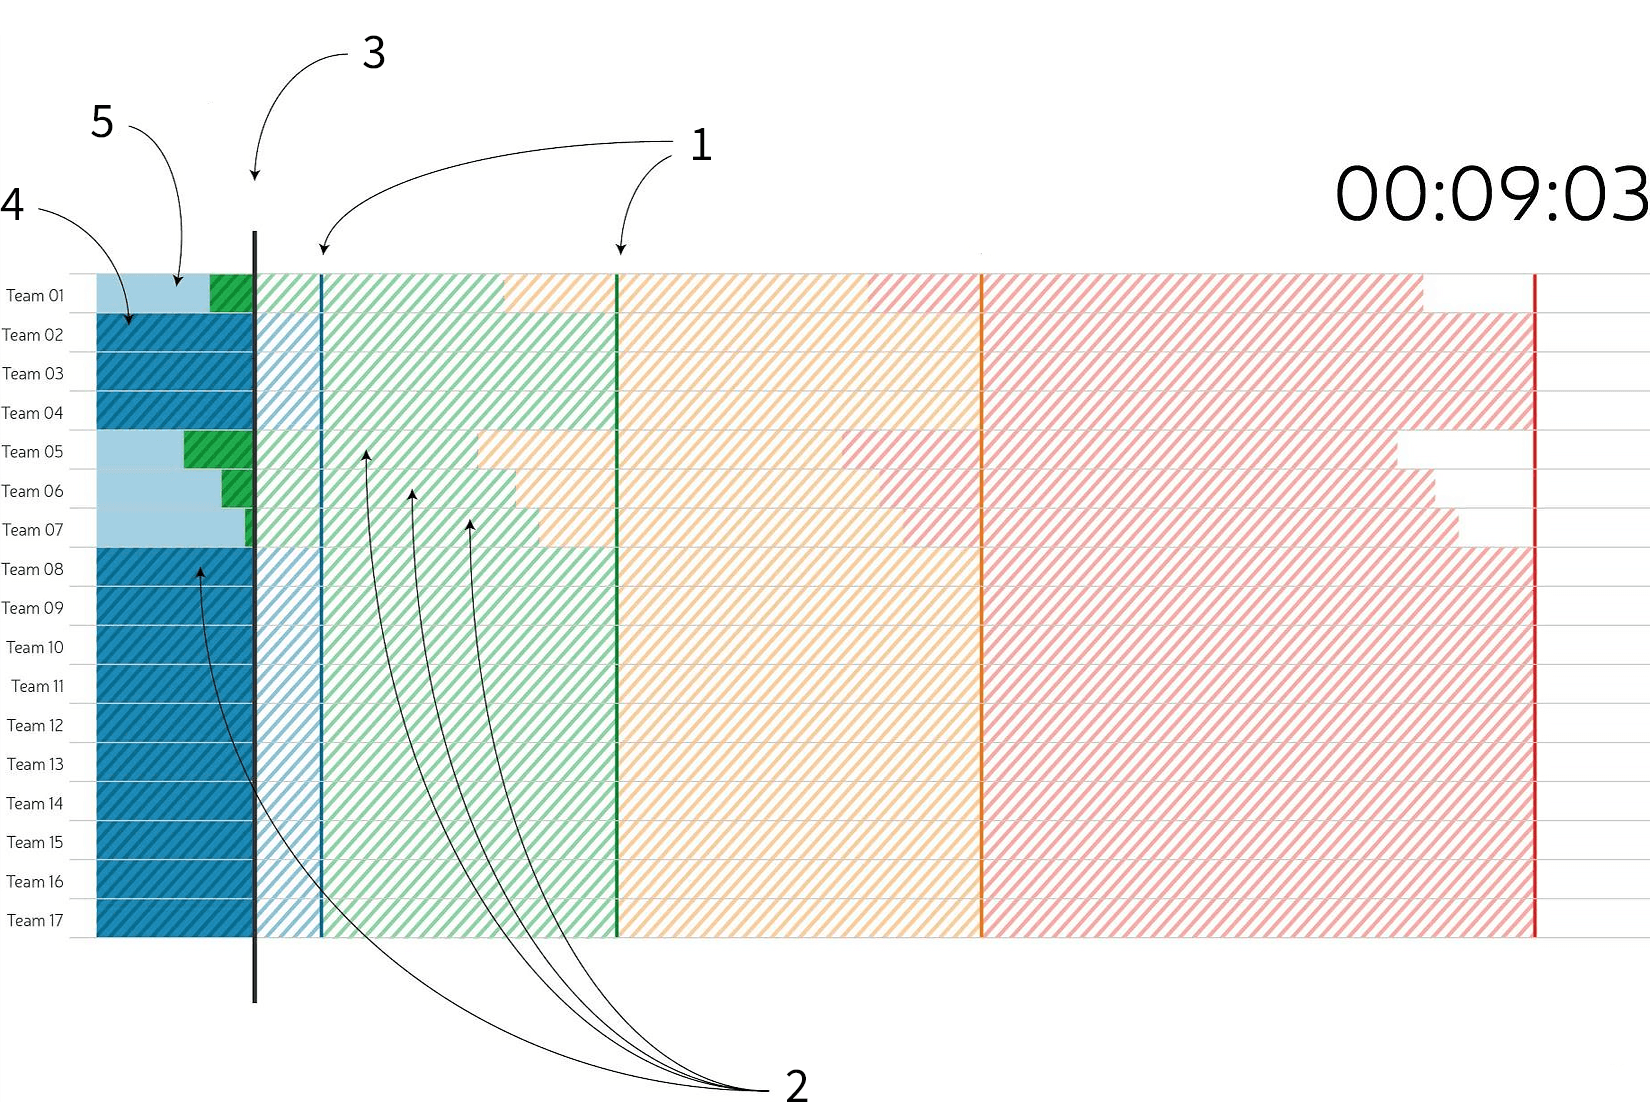
\includegraphics[width=12.7cm]{images/navrh-vizualizace-1-4.png}
  \end{center}
  \caption{Grafický návrh vizualizace od Bc.~Kristíny Zákopčanové, kde je znázorněn průběh hry po devíti minutách od jejího začátku.}
  \label{fig:progress1}
\end{figure}
Na obrázku \ref{fig:progress1} je znázorněn průběh hry krátce po jejím začátku společně s~odhadem času pro každou úroveň. Každému týmu přísluší jeden řádek, název týmu je uveden vlevo. Sloupce pak značí jednotlivé úrovně, které se odlišují svou barvou. V~pravém horním rohu se zobrazuje uplynulý čas.
\begin{enumerate}
  \item Svislé čáry představují odhadovanou dobu pro dokončení úrovně, jsou nezávislé na postupu týmu a~tudíž se nemění.
  \item Šrafovaná oblast vyznačuje předpokládanou dobu řešení úrovně pro daný tým. Její počátek je ovlivněn tím, kdy tým začal na úrovni pracovat, a~tedy také tím, kdy dokončil předchozí úrovně.
  \item Časová osa, která představuje aktuální moment.
  \item Sytější barva značí úroveň, na které tým právě pracuje.
  \item Světlejší barva značí již vyřešenou úroveň.
\end{enumerate}
\begin{figure}[H]
  \begin{center}
    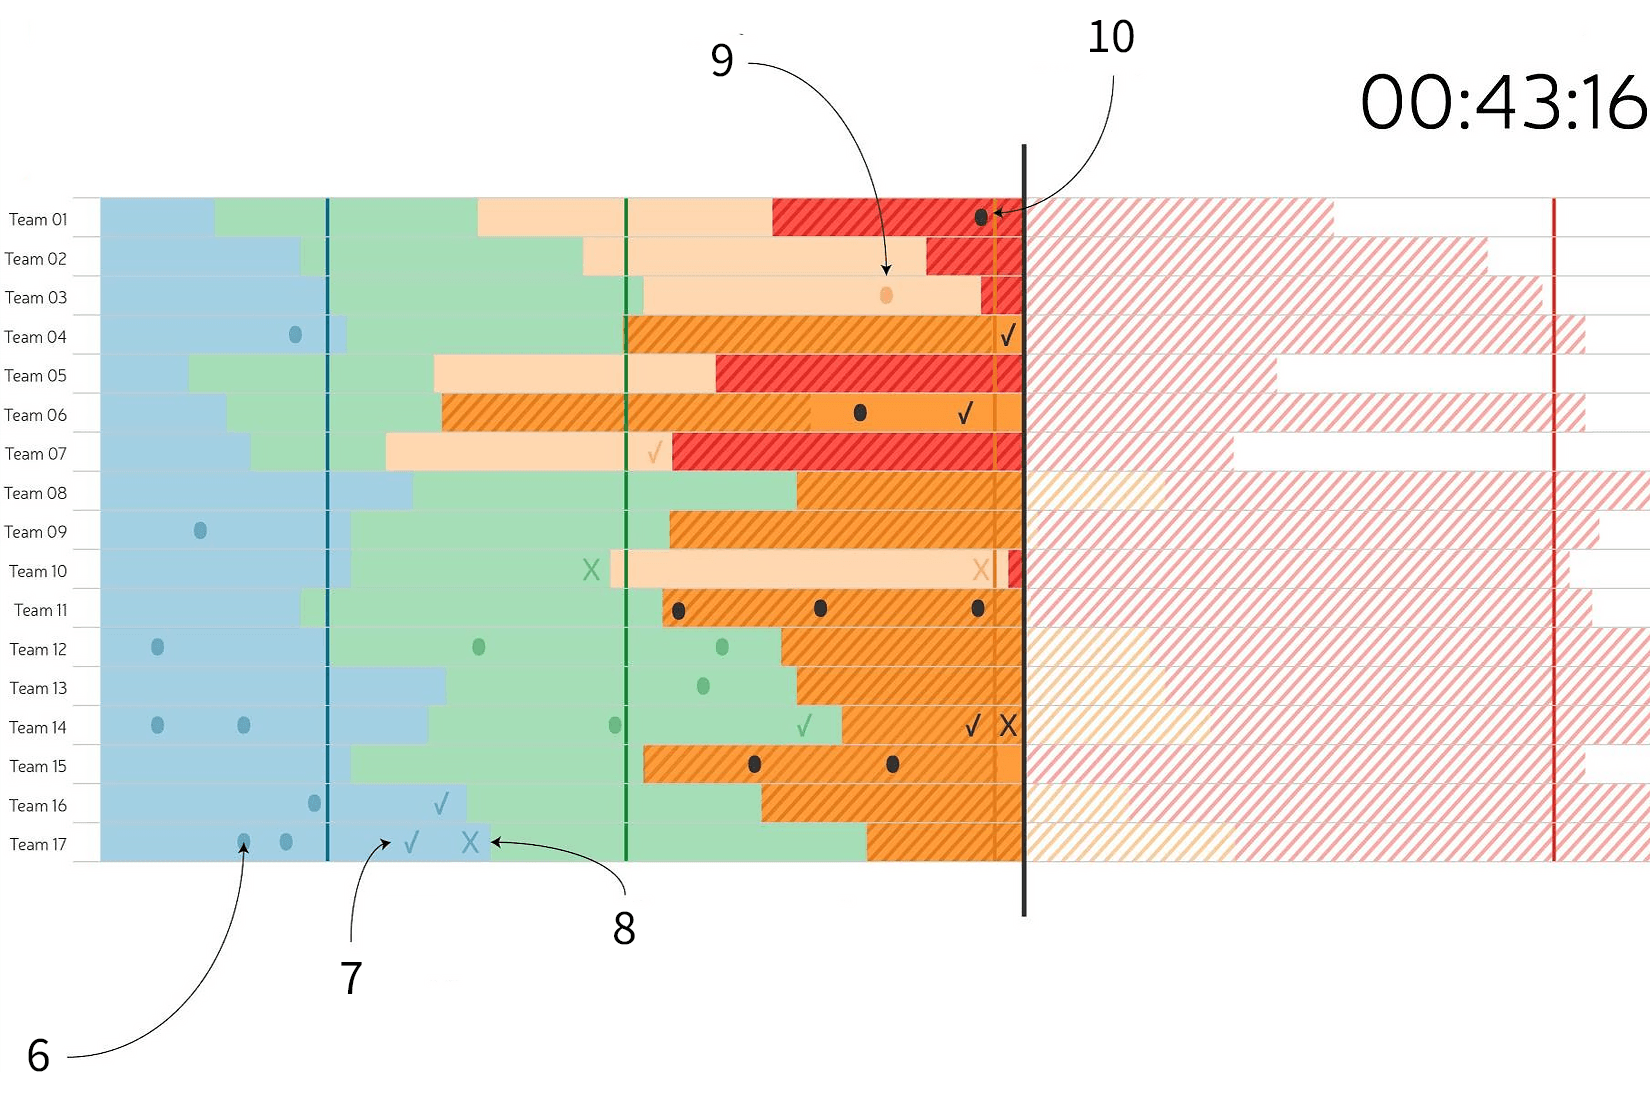
\includegraphics[width=12.7cm]{images/navrh-vizualizace-2-4.png}
  \end{center}
  \caption{Grafický návrh vizualizace od Bc.~Kristíny Zákopčanové, hra je za polovinou odhadované doby. Zobrazeny jsou i~jednotlivé události.}
  \label{fig:progress2}
\end{figure}
Návrh na obrázku \ref{fig:progress2} ukazuje další postup ve hře, kdy se již týmy nachází ve třetí nebo čtvrté úrovni. Navrženy jsou také události (6–8).
\begin{enumerate}
  \setcounter{enumi}{5}
  \item Tým využil nápovědu.
  \item Tým si zobrazil doporučené řešení úrovně.
  \item Tým úroveň přeskočil.
  \item V~již vyřešené úrovni jsou ikony v~podobném odstínu jako pozadí.
  \item V~aktuální úrovni jsou ikony tmavé a~výrazné z~důvodu lepší viditelnosti.
\end{enumerate}

\section{Požadavky na technologie a integraci} \label{technologyRequirements}
Z~hlediska použitých technologií a~integrace do projektu KYPO byly specifikovány následující požadavky:
\begin{itemize}
  \item bude se jednat o~webovou aplikaci,
  \item vizualizace bude ve formě Liferay portletu,
  \item základ aplikace bude v~podobě samostatného Angular~2 modulu,
  \item k~vizualizaci dat bude využita knihovna D3.js,
  \item aplikace bude schopná načítat data z~CSV souboru,
  \item dále bude schopná získávat data skrze REST API a~také tato data zobrazovat v~reálném čase.
\end{itemize}
KYPO využívá vlastní webový portál postavený na platformě Liferay, a~je tedy samozřejmým požadavkem, aby byla vizualizace součástí tohoto portálu jako samostatný portlet. Aplikace vizualizace má být implementována jako Angular modul, protože Angular byl vybrán jako jednotný framework pro vývoj dalších portletů do KYPO portálu a~také byla připravena kostra portletu využívající tento framework jako základ pro nové projekty. Samotná vizualizace má být vykreslována pomocí knihovny D3.js, která je určena právě pro vizualizaci dat.\par
Jako zdroj dat mají sloužit CSV soubory, popsané v~podkapitole o~rozšířeních CtF her \ref{gameExtensions}. Později, až bude k~dispozici API poskytující podobné záznamy událostí ze hry, má být aplikace schopná získávat data i~skrze toto rozhraní a~zobrazovat je v~reálném čase.
%%je to v reálném čase, když se jen každou sekundu překresluje?

\chapter{Použité technologie}
Na základě požadavků popsaných v~předchozí kapitole \ref{technologyRequirements} byly při implementaci použity následující technologie. Pro samotnou vizualizaci byla použita knihovna D3.js a~responzivní grid z~frameworku Bootstrap, aplikace je pak postavena na frameworku Angular. Načítání dat z~CSV souboru je řešeno pomocí knihovny Papa Parse, pro kterou existuje integrace do Angular aplikací. S~využitím již připraveného projektu v~rámci KYPO je pak tato aplikace integrována do Liferay portletu.

\section{D3.js}
%%vizuální reprezentace dat
D3.js (Data-Driven Document) je knihovna pro vizualizaci dat v~jazyce JavaScript. Poskytuje funkcionalitu potřebnou pro tvorbu webových vizualizací, které jsou zobrazitelné v~kterémkoliv moderním prohlížeči. Data-Driven značí, že jednotlivé prvky dokumentu jsou svázány s~daty a~jsou podle těchto dat vizuálně transformovány. \par
Knihovna je navržena jako kolekce spolupracujících modulů, které lze využívat i~samostaně \cite{d3APIReference}. Jednotlivé moduly jsou určeny například pro tvorbu základních tvarů, hierarchických struktur, pro práci s~barvami a měřítky, ale také pro animování a~různé interakce.
%Citace na github??????? d3APIReference

\subsection{Základ vizualizací}
D3.js nepřináší novou reprezentaci, ale využívá již existující standardy HTML, CSS a~SVG a~pouze pracuje se stávajícími prvky, které vytváří a~transformuje \cite{d3jsorg}. Základem vizualizací jsou právě SVG\footnote{SVG (Scalable Vector Graphics) je značkovací jazyk definující dvojrozměrnou vektorovou grafiku v~XML formátu. SVG kód lze vložit do kódu HTML stránky.} elementy.\par
SVG obsahuje elementy mnoha kategorií, patří mezi ně zejména různé kontejnery a~grafické prvky. \cite{svgMozillaorg}
\begin{itemize}
  \item Mezi obalující a~strukturální prvky patří např. \verb|<svg>| nebo \verb|<g>|. Značka \verb|<svg>| se používá pro vložení SVG grafiky do dokumentu, \verb|<g>| je kontejner používaný pro seskupení ostatních elementů. Oba dva prvky je možné zanořovat.
  \item Grafickými elementy jsou např. kruh \verb|<circle>|, obdélník \verb|<rect>|, úsečka \verb|<line>| nebo cesta \verb|<path>|, což je obecný element definující různé tvary.
	%%\begin{itemize}
	  %%\item Kruh \verb|<circle>| je definován svým středem se souřadnicemi \texttt{cx}, \texttt{cy} a poloměrem \texttt{r}.
	  %%\item Obdélník \verb|<rect>| je určen na základě pozice levého horního rohu \texttt{x} a \texttt{y}, šířky \texttt{width} a výšky \texttt{height}.
	  %%\item Úsečku \verb|<line>| definují dva koncové body \texttt{x1}, \texttt{y1} a \texttt{x2}, \texttt{y2}.
	  %%\item Cesta \verb|<path>| je oproti tomu obecný element definující různé tvary. Tvar určuje atribut \texttt{d}, což je textový řetězec tvořený kombinací instrukcí.
	%%\end{itemize}
\end{itemize}
%%využívá HTML, CSS a SVG, co je svg, příklady svg elementů - rectangle, circle, line, path

%%CSS selektory umožnují vybrat určité elementy DOM. Nejčastěji podle typu prvku nebo hodnoty jeho atributů (např. id nebo třídy).
\subsection{Princip práce s D3.js}
D3.js, podobně jako např. knihovna jQuery, pracuje a~manipuluje s~modelem dokumentu DOM\footnote{DOM (Document Object Model) je rozhraní pro XML a HTML dokumenty, které umožňuje přistupovat k~jednotlivým prvkům dokumentu a~měnit tak jeho strukturu, styl a~obsah. Jedná se o~objektově orientovanou reprezentaci stránky.}. V D3.js však mohou být styly a~atributy elementů specifikovány nejen jako konstanty, ale také jako funkce mapující data \cite{d3jsorg}.\par
Podstatou je mapování dat na jednotlivé vlastnosti elementů vizualizace. Tím jsou elementy transformovány, ať už je to jejich velikost, poloha, barva atd. Jakým způsobem se data budou mapovat, záleží na vlastní implementaci a~na typu vybraného grafu. Například u~sloupcového grafu budou data ovlivňovat výšku sloupců, u~bublinového zase poloměr či polohu kruhů. \cite{interactiveVisualizationBook}\par
Princip vykreslování jednotlivých prvků vizualizace je následující:
\begin{itemize}
  \item výběr množiny uzlů,
  \item mapování dat na vybranou množinu,
  \item případné vytvoření chybějících (nebo vymazání přebytečných) uzlů,
  \item transformace elementů podle namapovaných dat.
\end{itemize}
Nejdříve je nutné vybrat prvky dokumentu, které se sváží s~daty. Pokud dosud neexistují, budou vytvořeny (třetí krok). Konkrétní výběr se určí pomocí CSS selektoru.
%popsat css selektor
Lze vybírat jeden samotný uzel pomocí metody \verb|select|, nebo množinu všech uzlů odpovídajících danému selektoru pomocí \verb|selectAll|. Následující příkaz označí všechny obdélníky \verb|<rect>|.
\begin{markdown*}{
  fencedCode
}
``` sh
	d3.selectAll("rect"); 
```
\end{markdown*}
Data se vkládají metodou \verb|data|. Pokud se jedná o~pouhou aktualizaci již existujících elementů, další krok není potřebný a~mohou být přímo aplikovány transformace. Ukázka vložení pole s daty a~změna výšky obdélníků podle těchto dat:
\begin{markdown*}{
  fencedCode
}
``` sh
	d3.select("svg").selectAll("rect")
	  .data([5, 10, 15, 20, 25])
	  .attr("height", function(d) { return d; });
```
\end{markdown*}
V případě, že elementy dosud neexistují (nebo je jejich počet menší, než délka datového pole), jsou chybějící elementy přidány voláním metod \verb|enter| a \verb|append|.
\begin{markdown*}{
  fencedCode
}
``` sh
	d3.select("svg").selectAll("rect")
	  .data([5, 10, 15, 20, 25])
	  .enter().append("rect")
	  .attr("height", function(d) { return d; });
```
\end{markdown*}
\subsection{Příklady grafů a vizualizací}\label{d3jsGraphs}
Knihovna poskytuje pouze potřebnou funkcionalitu pro vizualizaci dat, připravené vizualizace v~D3.js nejsou. K dispozici je však několik metod, které usnadní práci s~určitými typy vizualizací a~grafů. Metoda předaná data transformuje, přepočítá a~vrátí obecně složitější datovou strukturu, která je vhodná pro určitý druh vizualizace. Následuje několik příkladů možných využití knihovny. \cite{d3APIReference}
\begin{itemize}
  \item Line generuje aproximace křivek a lomené čáry (spline, poly\-line) pro použití ve spojnicových grafech.
  \item Area počítá plochy pro použití v~plošných grafech, definované dvěma ohraničujícími čarami.
  \item Pie vypočítává potřebné úhly pro výsečové nebo prstencové grafy. Pomocí \verb|arc| pak mohou být na základě těchto úhlů vygenerovány oblouky grafu.
  \item Stack slouží pro tvorbu skládaných sloupcových grafů (obr. \ref{fig:stackBarChart}). Data obsahují klíče, kterými se specifikují dané vrstvy:
\begin{markdown*}{
  fencedCode
}
```
	[{ apples: 5, oranges: 10, grapes: 22 },
	{ apples: 4, oranges: 12, grapes: 28 }]
```
\end{markdown*}
  \item Histogram je součástí modulu pro práci s~poli a~počítá histogram pro zadané pole vzorků.
  \item Force je modul určený pro zjednodušenou simulaci působení fyzikálních sil na jednotlivé prvky. Pracuje se s~daty jako u~orientovaných grafů, tj. s~vrcholy spojenými orientovanými hranami:
\begin{markdown*}{
  fencedCode
}
```
	nodes = [{ name: "Alice" }, { name: "Bob" }];
	edges = [{ source: 0, target: 1 },
			 { source: 1, target: 0 }];
```
\end{markdown*}
\begin{figure}[H]
  \begin{center}
    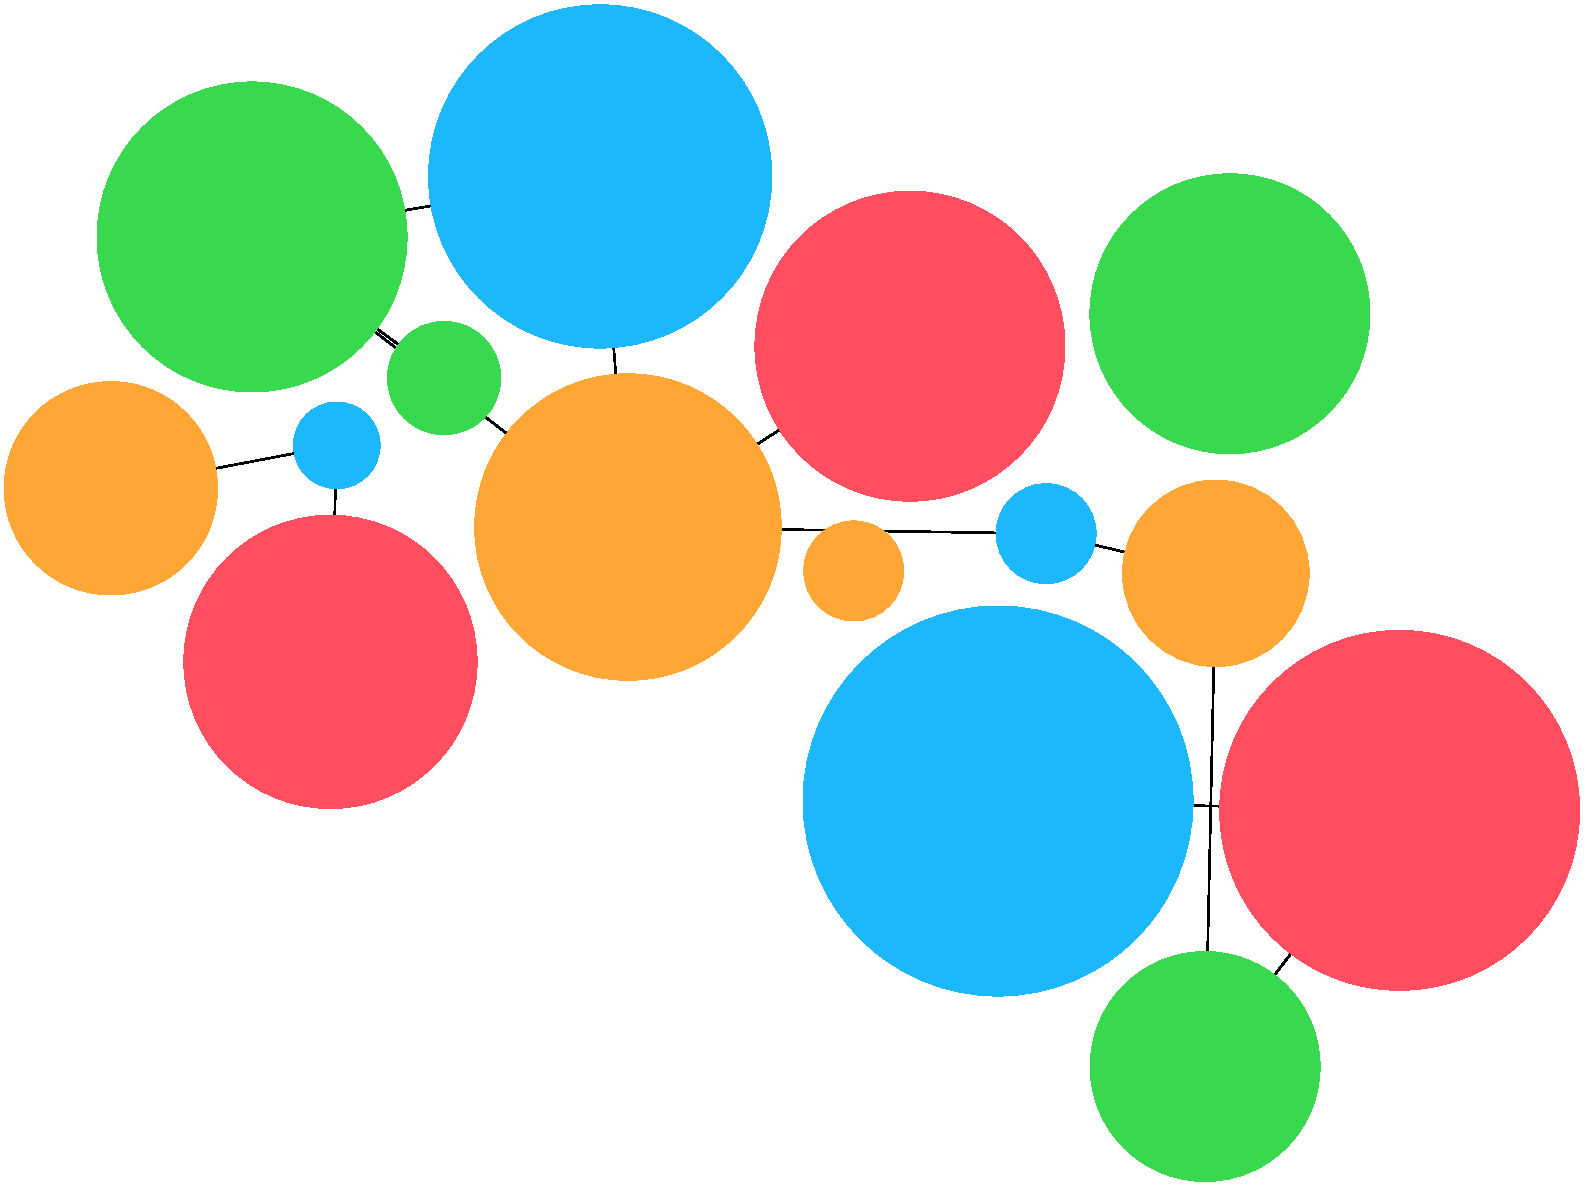
\includegraphics[width=3.7cm]{images/force.pdf}
  \end{center}
  \caption{Graf vytvořený s využitím modulu \texttt{d3-force}.}
  \label{fig:forceGraph}
\end{figure}
  \item Pack patří do modulu pro práci s~hierarchickými daty. Hierarchie je reprezentována zanořením, kvantita velikostí prvků. Uzel stromu je reprezentován jako kruh, obsahující uvnitř své podstromy jako menší kruhy. Velikost uzlu aproximuje součet velikostí jeho podstromů.
\end{itemize}

\begin{figure}[H]
  \RawFloats
  \centering
  \begin{minipage}[b]{0.35\textwidth}
  	\centering
    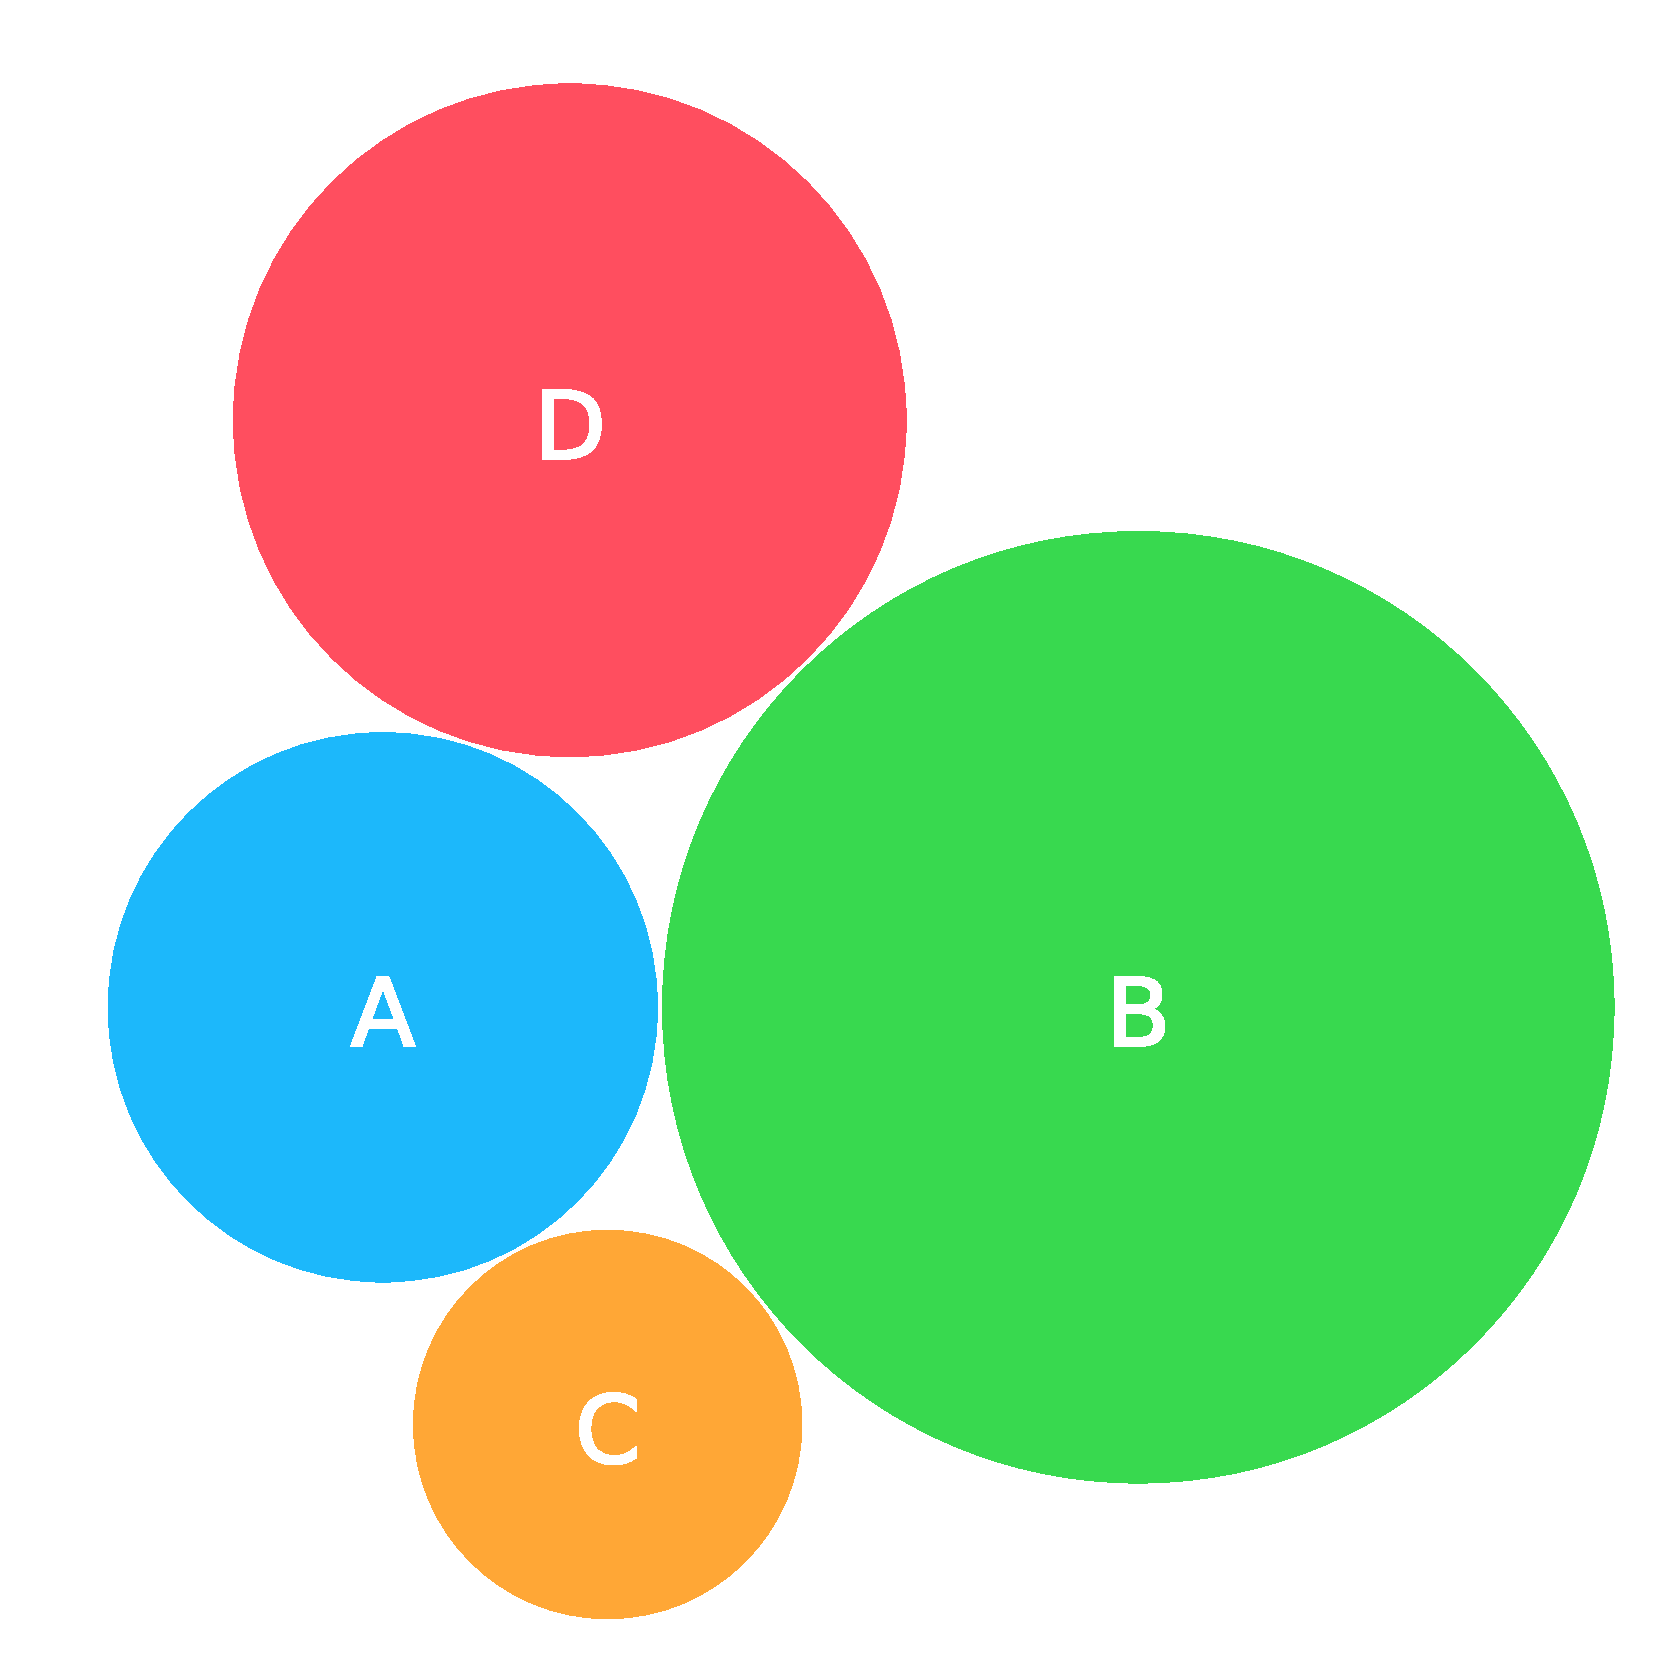
\includegraphics[width=\textwidth]{images/bubble.pdf}
    \caption{Bublinový graf vytvořený pomocí \texttt{d3.pack}.}
    \label{fig:bubbleChart}
  \end{minipage}
  \hfill
  \begin{minipage}[b]{0.5\textwidth}
    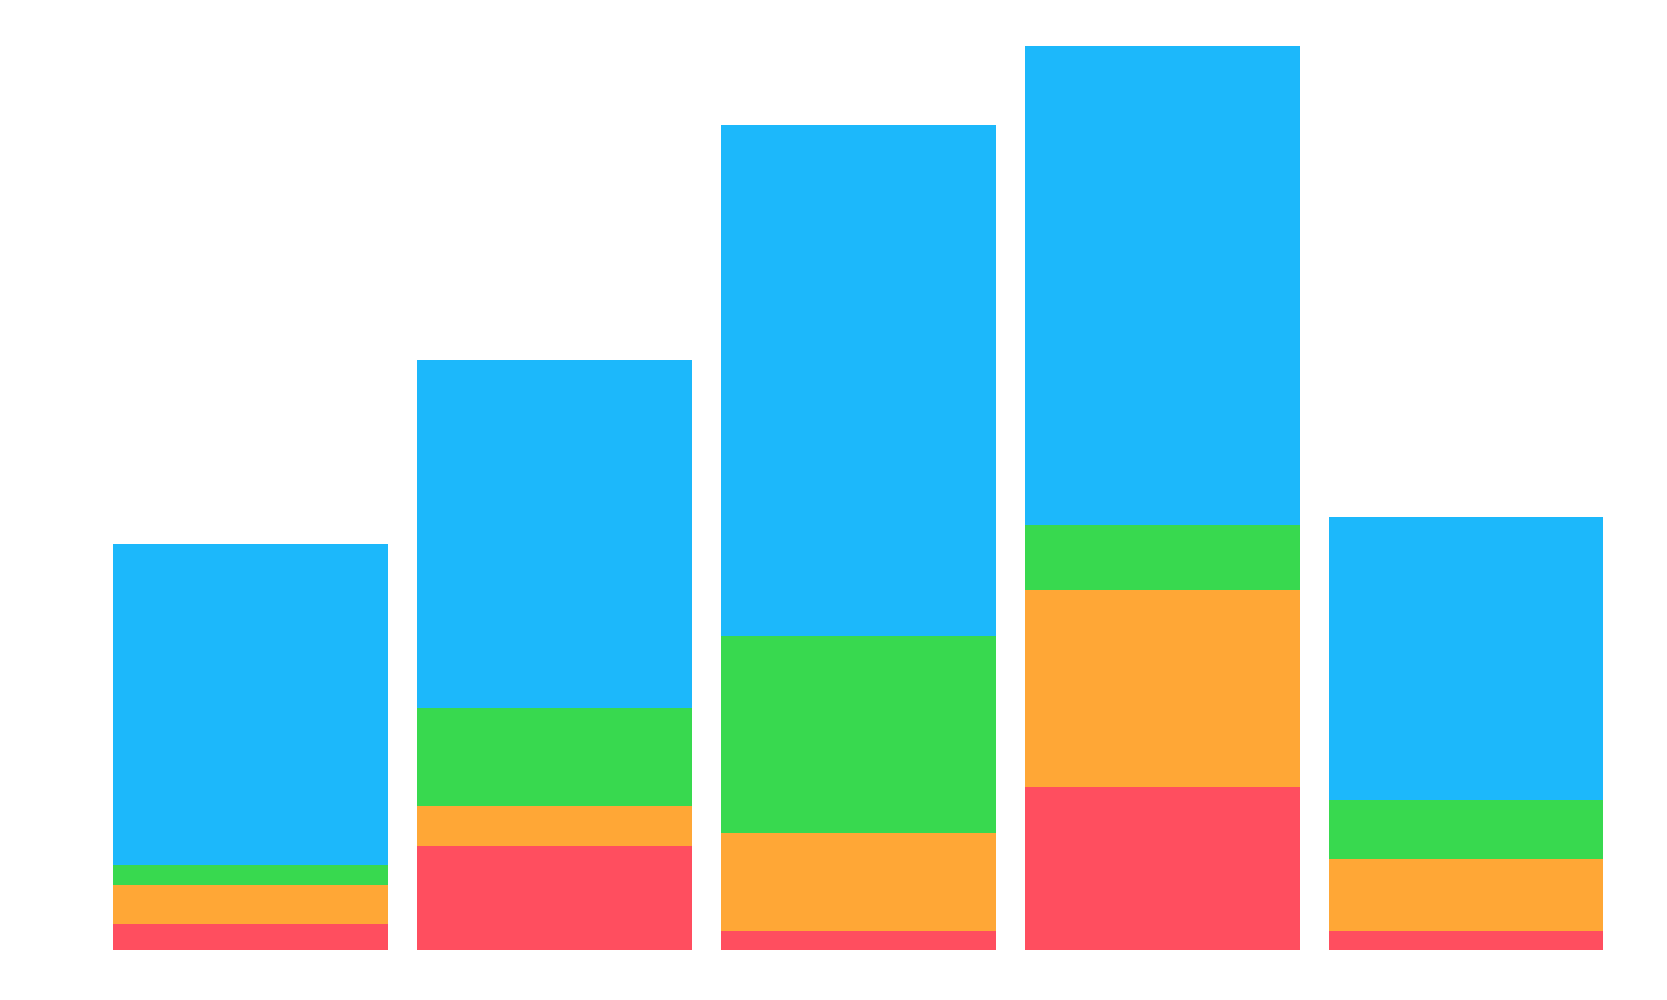
\includegraphics[width=\textwidth]{images/stack.pdf}
    \caption{Skládáný sloupcový graf (stacked bar) vytvořený s~využitím \texttt{d3.stack}.}
    \label{fig:stackBarChart}
  \end{minipage}
\end{figure}

\section{Bootstrap}
Bootstrap je framework určený pro tvorbu responzivních webových stránek, který zahrnuje řadu stylů a~UI komponent usnadňujících vývoj v~HTML a~CSS. Tvoří jej sada CSS stylů, některé komponenty ale vyžadují také JavaScript.\par
Framework tvoří například následující součásti: \cite{bootstrapcom}
\begin{itemize}
  \item responzivní gridový systém pro rozložení stránky,
  \item obecné styly např. pro pozicování, odsazení, viditelnost elementů apod.,
  \item styly pro obsahové prvky, např. text (zarovnání textu, tloušťka písma), tabulky nebo responzivní obrázky,
  \item komponenty, jako např. navigace, modalová okna, formuláře, stránkování, rozbalovací nabídky atd.
\end{itemize}
Boostrap je jednoduše dostupný ve formě zkompilovaných CSS a~JS souborů, je ale také možné použít zdrojové soubory (Sass\footnote{Sass (Syntactically Awesome StyleSheets) je jedním z~CSS preprocesorů, který rozšiřuje možnosti CSS stylů např. o~proměnné, zanořování, funkce, cykly apod., čímž ulehčuje práci a~údržbu a~zmenšuje množství potřebného kódu. Kód se kompiluje do výsledného CSS souboru.} a~JavaScript). V~druhém případě je nutné zdroje kompilovat, je ale možné je zařadit do vlastního projektu a~kompilovat všechny zdroje jako celek. Lze pak například použít jen potřebné komponenty a~přizpůsobovat framework vlastním potřebám.

\subsection{Gridový systém}
Gridový systém slouží k~rozložení a~zarovnání obsahu stránky. Používá se jako série kontejneru, řádků a~sloupců. \cite{bootstrapcom} Kontejner obaluje obsah stránky a~centruje ho. Do kontejneru patří řádky, které vždy obalují sadu sloupců. Sloupce mohou být v~libovolných kombinacích, až 12~sloupců na řádek, pak se zalamují. Řádky se sloupci lze libovolně zanořovat do jiných sloupců.\par
Grid je responzivní a~je definováno několik mezí rozlišení v~pixel\-ech, které odpovídají určitým typům zařízení (mobilní telefon na výšku a~na šířku, tablet, notebook a~velké obrazovky). Počet sloupců na řádku se dá specifikovat pro tyto meze zvlášť, např. čtyři sloupce, které jsou vedle sebe na velké obrazovce, se na mobilním zařízení zalomí po jednom pod sebe.

\section{Angular}
\section{Papa Parse}
\section{Liferay} \label{liferay}

\chapter{Implementace}
Prvním krokem při implementaci bylo vytvoření základu vizualizace v D3.js, což zahrnuje především výběr vhodného typu grafu (příklady jsou uvedeny v kapitole \ref{d3jsGraphs} o D3.js), návrh datové struktury, vykreslení všech požadovaných prvků vizualizace a načtení dat z CSV souboru.\par
V dalším kroku byla vizualizace integrována do Angular aplikace jako samostatný modul, byly přidány interaktivní prvky a také načítání dat skrze API. O vytvoření Lifereay portletu s Angular aplikací se již stará skript, který připravil Bc. David Beran v rámci projektu \verb|kypo2-portlet-empty-angular|.
% zeptat se jestli jen David Beran
\section{Základ vizualizace}
Jako základní struktura pro stavbu vizualizace byl vybrán skládaný sloupcový graf, tzv. stacked bar chart (obr. \ref{fig:stackBarChart}). Ten má několik vrstev položených na sebe. V tomto případě se přesněji jedná o graf pruhový, jelikož bylo nutné jej pro vizualizaci otočit a vykreslovat jako horizontální pruhy.\par
V knihovně D3.js existuje pro tento typ grafu soubor metod s názvem Stack, který je částí modulu pro grafická primitiva \verb|d3-shapes|. Stack lze obecně použít pro tvary, které mají být na sebe těsně naskládány, mohou být takto skládány i plošné grafy. Negeneruje graf nebo tvary přímo, ale vypočítává pozice, podle kterých lze následně tvary vykreslit. \cite{d3jsorg}\par

\subsection{Základ grafu pro vizualizaci} \label{chartBase}
Tento typ grafu lze chápat jako několik vrstev, které jsou vertikálně naskládány na sebe, nebo jako v tomto případě vedle sebe.
\begin{figure}[H]
  \begin{center}
    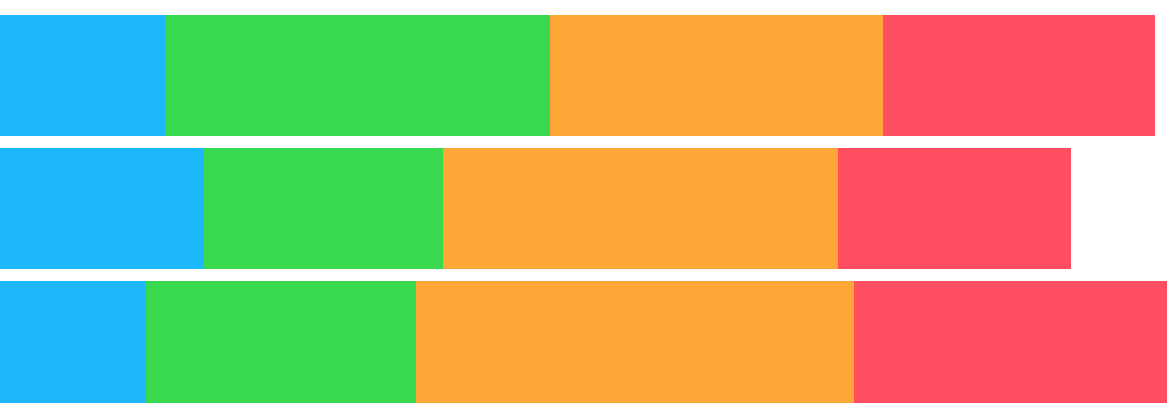
\includegraphics[width=4cm]{images/stack-ctf.pdf}
  \end{center}
  \caption{Využití skládaného grafu pro vizualizaci herních úrovní.}
  \label{fig:visualizationChart}
\end{figure}
Každá vrstva grafu představuje určitou kategorii identifikovanou vlastním klíčem. Jednotlivými kategoriemi budou v této vizualizaci úrovně hry s odpovídajícími klíči \verb|level1|, \verb|level2|, \verb|level3| atd. Jejich hodnota bude vždy čas, který tým v dané úrovni strávil, počítaný v sekundách. Příklad struktury dat pro dva týmy a tři herní úrovně:
%[{"team": 1, "level1": 850, "level2": 740, "level3": 910},
% {"team": 2, "level1": 630, "level2": 950, "level3": 980}]
\begin{markdown*}{
  fencedCode
}
```Java
	[{"team": 1, "level1": 850, "level2": 740},
	 {"team": 2, "level1": 630, "level2": 950}]
```
\end{markdown*}

Struktura potřebná pro vykreslení SVG elementů je z takových dat vypočítána pomocí \verb|stack| z D3.js. Je třeba specifikovat klíče, podle nich se pak data seskupí a vypočítají se pozice jednotlivých vrstev.

\begin{markdown*}{
  fencedCode
}
```Java
	stack = d3.stack()
			  .keys(["level1", "level2"])
	layers = stack(data);
```
\end{markdown*}
Vráceno je pole, jehož prvky reprezentují jednotlivé kategorie, tedy herní úrovně. Každá úroveň je opět pole a jeho prvky odpovídají jednotlivým týmům.
%[[[   0, 850], [   0, 630]],        // level1
%	  [[850, 1590], [630, 1580]],       // level2
%	  [[1590, 2500], [1580, 2560]]]     // level3
\begin{markdown*}{
  fencedCode
}
```Java
	[[[   0, 850], [   0, 630]],     // level1
	  [[850, 1590], [630, 1580]]]    // level2
```
\end{markdown*}
%ZRUŠIT ODSAZENÍ PŘED KÓDEM?????????????????????????
Vypočítané hodnoty již vymezují jednotlivé úrovně v grafu, v tomto případě jejich \mbox{x-ové} pozice pro každý tým. Hodnota na ose y se určí dle týmu. Na základě těchto hodnot už mohou být vykresleny jednotlivé SVG obdélníky \verb|<rect>| do grafu.

\subsection{Měřítka}
Data mohou nabývat hodnot v různém rozsahu a je nutné je při vykreslování vhodně škálovat do výsledného obrazu. Měřítka (scales) v D3.js jsou funkce, které mapují hodnoty z domény vstupních dat do výstupního rozsahu vizualizace \cite{d3jsorg}. Měřítek je několik v závislosti na vstupní doméně a výstupním oboru hodnot. Pro tuto vizualizaci jsou podstatné následující dva typy:
%do výstupních rozměrů vizualizace?
%do výstupního obrazu?
\begin{itemize}
  \item spojitá měřítka, která mapují hodnoty ze spojité číselné domény do spojitého oboru hodnot,
  \item ordinální měřítka pro mapování diskrétních hodnot na diskrétní.
\end{itemize}
Osa x vizualizace představuje čas a bylo pro ni použito spojité měřítko, konkrétně lineární \verb|d3.scaleLinear|, aby byl čas mapován rovnoměrně.\par
Na ose y se nachází jednotlivé týmy. Týmy tvoří diskrétní množinu, stejně jako jednotlivé řádky vizualizace. Proto bylo použito měřítko ordinální, konkrétně se jedná o \verb|d3.scaleBand|, které každý tým mapuje podle jména na správný řádek vizualizace.
%Na ose y se nachází jednotlivé týmy a proto bylo nutné použít měřítko ordinální.

\subsection{Barvy}

\section{Datová struktura}
%Dalším důležitým krokem byl návrh datové struktury, se kterou má vizualizace pracovat. Ta musí obsahovat všechny potřebné informace tak, aby mohly být vykresleny všechny požadované prvky ze zadnání, např. aktuální čas od začátku hry, data jednotlivých hráčů nebo časový plán. Některá data pak musí být v určitém formátu, jako např. strávený čas v jednotlivých úrovních, který musí mít formát popsaný v předchozí podkapitole, aby mohl být vypočítán a vykreslen skládaný graf. Dle toho byla navržena následující datová struktura, se kterou vizualizace pracuje:
Záznamy událostí ze hry, ať už ve formátu CSV nebo JSON, musí být nejdříve zpracovány do vhodné datové struktury, se kterou bude vizualizace pracovat. Některá data musí být v určitém formátu, aby mohla být zprácována za pomoci \verb|d3.stack| do výsledného grafu. Jedná se o odhadovanou a skutečnou délku každé úrovně pro jednotlivé týmy. Některé údaje musí být ze záznamů vypočítány.\par Datová struktura, se kterou vizualizace pracuje, je objekt s těmito atributy:
\begin{itemize}
  \item \verb|time| – časové razítko udávající čas od začátku hry v sekundách,
  \item \verb|levels| – pole klíčů jednotlivých úrovní hry,
  \item \verb|levelsTimePlan| – pole čísel udávájící časový odhad pro každou úroveň v sekundách,
  \item \verb|gameDataset| – pole objektů představující týmy, má popsanou strukturu potřebnou pro použití s \verb|d3.stack|, uchovává však některé informace navíc:
  	\begin{itemize}
		\item \verb|team| – název týmu,
		\item \verb|startTime| – čas v sekundách, kdy tým začal hru
		\item \verb|totalTime| – celkový čas, který již tým strávil ve hře
		\item \verb|currentState| – aktuální úroveň, na které tým právě pracuje
		\item \verb|events| – pole událostí, jako využité nápovědy, zobrazená řešení nebo přeskočení úrovně
		\item \verb|level1|, \verb|level2|, \verb|level3|… čas strávený v jednotlivých úrovních, pro zpracování pomocí d3.stack do skládaného grafu,
	\end{itemize}
  \item \verb|planDataset| – podobné pole objektů jako \verb|gameDataset|, avšak bez některých prvků, používá se pro vykreslení časového plánu hry.
\end{itemize}
%, jako využité nápovědy, celkově strávený čas apod.,

\section{Struktura vizualizace}
%K celkovému rozložení na stránce byl použit grid z frameworku Bootstrap, který vizualizaci centruje a zarovnává některé její prvky.
Vizualizace se skládá z několika částí, které se vykreslují postupně. K celkovému rozložení na stránce byl použit grid z frameworku Bootstrap.
%dát to víc do gridu, např. selecty, aby se dalo napsat, že je díky gridu responzivní

\begin{figure}[H]
  \begin{center}
    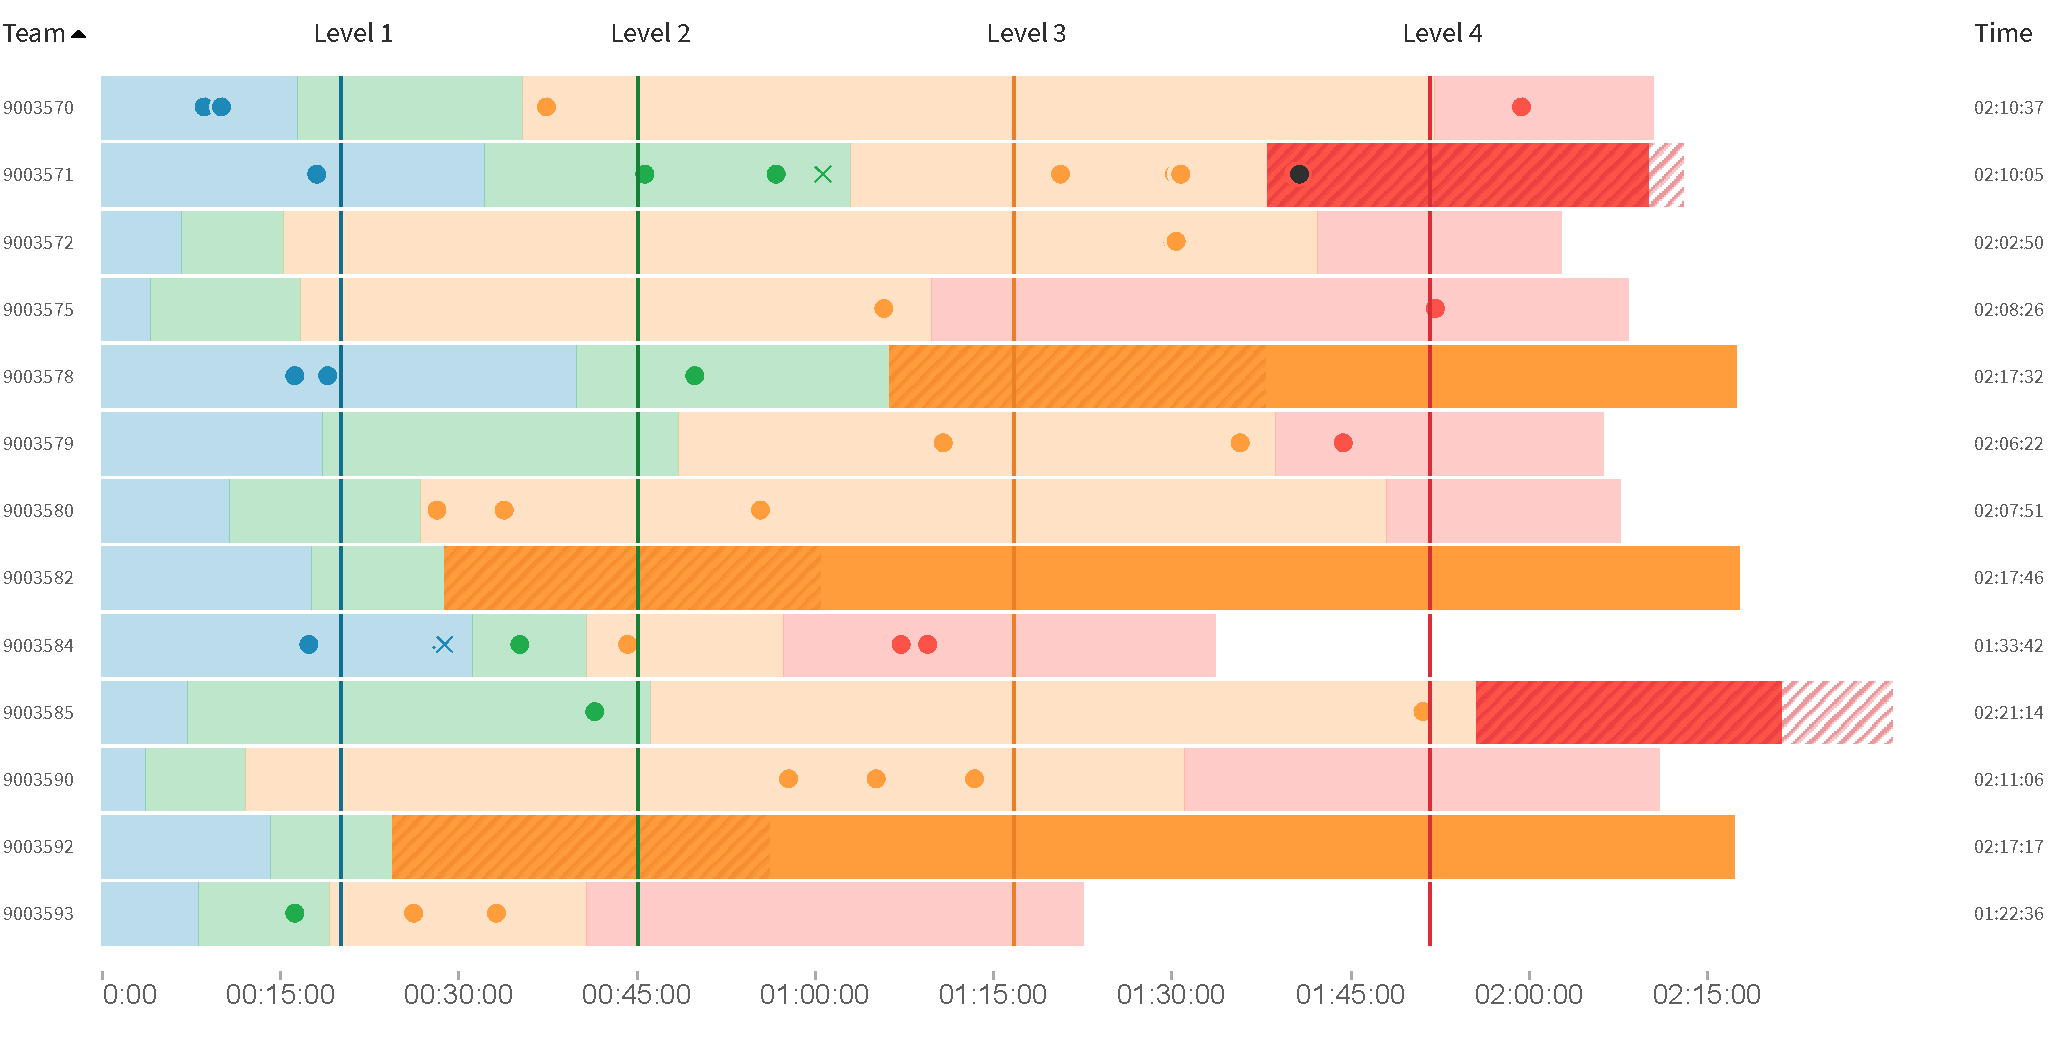
\includegraphics[width=12.7cm]{images/ctf-all.pdf}
  \end{center}
  \caption{Implementovaná vizualizace s reálnými daty z CSV souboru.}
  \label{fig:visualizationChart}
\end{figure}
%OBRÁZEK DÁT Z PROGRESS VIEW!!!!!!!!!!!!!!!!!!!!!!!!!!!!!!!!!!!!!!!!!!!!!!! aby tam byl čas!!!!!!!!!!!!!!!!

% Tento element zahrnuje vizualizaci časového plánu hry, vizualizaci skutečné délky úrovní, události v podobě ikon, osu x a časovou osu vyznačující aktuální okamžik v grafu.
Hlavní část vizualizace je v rámci jednoho SVG elementu. Tento element zahrnuje:
\begin{enumerate}
  \item vizualizaci časového plánu hry,
  \item vizualizaci skutečné délky úrovní,
  \item události v podobě ikon,
  \item osu x,
  \item časovou osu vyznačující aktuální okamžik v grafu.
\end{enumerate}

\begin{markdown*}{
  fencedCode
}
```HTML
	<svg class="ctf-progress-chart">
	   <g class="ctf-game-wrapper">
	      <g class="ctf-game">
	         <g class="axis-x">...</g>		  //4
	         <g class="game">...</g>		  //2
	         <g class="plan">...</g>		  //1
	         <g class="events">...</g>		  //3
	         <g class="bounds">...</g>		  //1
	         <line class="timeline"></line>	  //5
	      </g>
	   </g>
	</svg>
```
\end{markdown*}

Ostatní elementy, jako názvy a celkový čas týmů nebo text ukazující aktuální čas, jsou umístěny zvlášť v samostatných sloupcích okolo vizualizace.

%ukazka struktury svg ve sbalenem kodu --> struktura vygenerovaneho svg kodu vizualizaci
\subsection{Základní prvky vizualizace}
Nejdříve je vygenerován nutný základ vizualizace, především hlavní \verb|<svg>| element, ale také obalující \verb|<g>| elementy.\par
Šířka \verb|<svg>| je vypočítána na základě šířky rodičovského HTML elementu a odvíjí se od toho, jakou šířku má viewport\footnote{Viewport je zde oblast, do které prohlížeč vykresluje stránku, tedy viditelná část webové stránky.}. Výpočet výšky závisí na více proměnných. Při výpočtu je brána v úvahu výška viewportu, počet týmů a minimální přednastavená výška jednoho řádku vizualizace. Závisí ale také na vypočítané šířce, a to z důvodu částečného zachování proporcí.\par
Dále jsou vytvořena a nastavena měřítka pro obě osy x a y. Doménou x-ového měřítka je celková odhadovaná délka hry, pro y je to množina týmů.\par
V této části je taaké je vykreslena osa x, hustota bodů na této ose respektuje šířku vizualizace. Osa y se nevykresluje, její úlohu plní sloupec s názvy týmů na levé straně, který umožňuje řazení řádků.
%zjemňuje se při zoomování?! dodělat
%vyznačit nějak x a y?

\subsection{Vizualizace časového plánu}
\begin{figure}[H]
  \begin{center}
    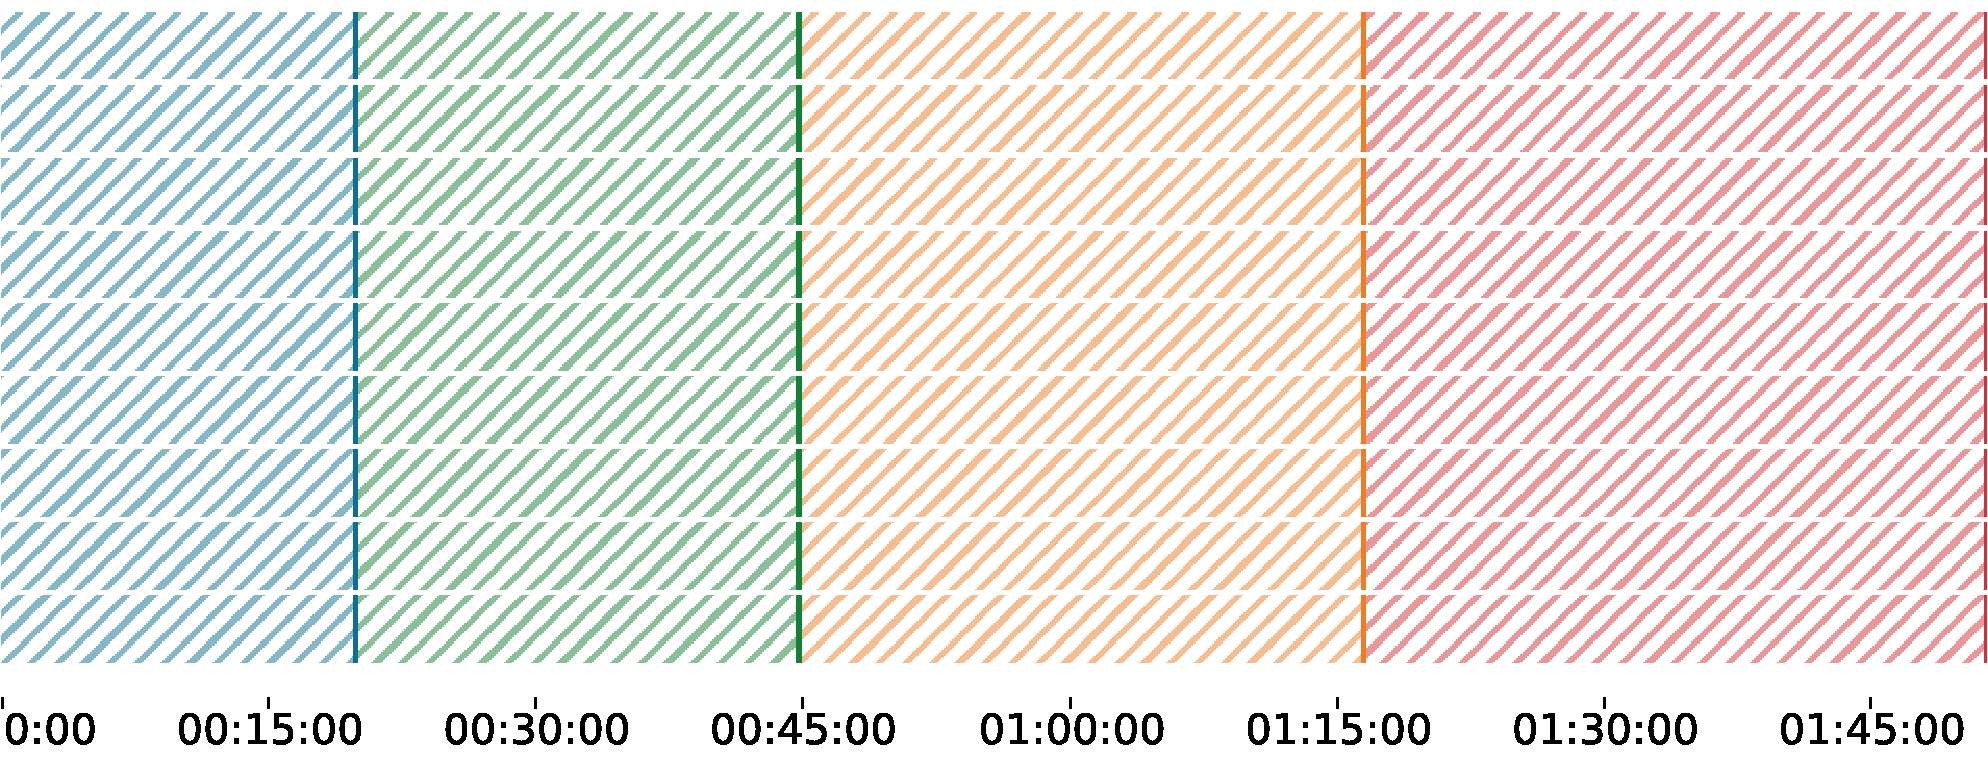
\includegraphics[width=12.7cm]{images/ctf-plan.pdf}
  \end{center}
  \caption{Časový odhad jednotlivých úrovní. Svislé čáry znázorňují nezávislý odhadovaný limit. Šrafované oblasti se týkají vždy daného týmu a jejich začátek se posunuje v závislosti na postupu týmu.}
  \label{fig:visualizationChart}
\end{figure}
Odhadovaný časový limit pro jednotlivé úrovně je vykreslován způsobem popsaným v podkapitole o základu grafu \ref{chartBase}. Použitá datová struktura je stejná, ale místo skutečného postupu týmů je v ní v ní uložen pouze odhad:
\begin{markdown*}{
  fencedCode
}
```Java
[{"team": 1, "level1": 1000, "level2": 2000}]
```
\end{markdown*}
Vykreslování probíhá dvakrát, nejdříve jsou pomocí d3.stack vygenerovány šrafované obdélníky a poté hranice v podobě svislých čar.

\subsection{Vizualizace herních úrovní}
Princip vykreslování skutečné délky úrovní je opět stejný jako již popsaný způsob v \ref{chartBase}. Během vykreslování je však navíc třeba brát v úvahu, zda již tým úroveň dokončil, nebo na ní právě pracuje, kvůli přidělení světlé nebo syté barvy. Tato informace je již předpočítána v datové struktuře.\par
Jelikož týmy již mohly překročit celkový odhad a graf by přesáhl stanovenou šířku vizualizace, je nutné před vykreslením aktualizovat měřítka.\par
Po vykreslení reálných dat je třeba aktualizovat plán. Mohlo dojít ke změně měřítka a také je nutné posunout šrafované oblasti, které jsou závislé na aktuálním postupu týmu. Všechny šrafované oblasti s výjimkou té, která se týká aktuální úrovně, jsou skryty. Šrafování týkající se aktuální úrovně je posunuto na její začátek.
%% byly přidány další levely a je jich teď 6 -> ukázka s 6 levely
\subsection{Události}
Po zobrazení plánu a postupu týmů se vykreslují jednotlivé události v podobě ikon. Každý objekt události nese informace o svém čase, týmu i úrovni, podle kterých je vykreslen do grafu. Uchovává také typ události, podle kterého je zvolen tvar ikony.
%POSUNOVÁNÍ PŘI ZMĚNĚ POHLEDU!
\subsection{Sloupce s údaji}
Informace vztahující k jednotlivým řádkům jsou zaznamenány v okolních sloupcích. Prvním z nich je sloupec s názvy týmů na levé straně, ten zároveň zastupuje osu y. Druhý sloupec na pravé straně udává celkový čas, který již tým ve hře strávil.\par
Nad těmito sloupci je umožněno řazení a jsou zarovnány se souvisejícími ovládacími prvky. Z tohoto důvodu jsou umístěny mimo hlavní <svg> element vizualizace.\par
Přidání dalších sloupů na pravou stranu je možné. Mohly by být přidány například informace o bodovém hodnocení, pokud budou k dispozici odpovídající data.
%možné přidat další sloupce
\subsection{Další prvky}
Mezi další součásti vizualizace patří tyto prvky:
\begin{itemize}
  \item časová osa, která je vykreslena jako čára v místě aktuálního okamžiku,
  \item čas od začátku hry v pravém horním rohu, převádí se z časového razítka v datové struktuře,
  \item popisky zobrazující se po najetí na ikonu události.
\end{itemize}
Popisky událostí jsou řešeny jako jediný element, který je při najetí na událost přesunut na její pozici a odkryt. Zároveň je změněn jeho text podle popisu dané události.

\section{Pohledy vizualizace}
Během implementace bylo zjištěno, že týmy nezačínají hru ve stejný okamžik, což znamená změnu oproti grafickému návrhu. Ten vychází z předpokladu, že týmy začínají hru stejně, a řádky jsou proto z levé strany zarovnány, což neodpovídá skutečnosti. Tento pohled je však užitečný, protože lze porovnávat dobu řešení úrovně s časovým limitem, který je naznačen svislou čarou. Také lze tímto způsobem jednodušeji porovnávat týmy mezi sebou.\par
Jednotlivé řádky je možné zarovnat podle jejich počátku, jako je tomu v grafickém návrhu. Dojde tak ale k jejich posunutí a řádky přestanou být zarovnány s časovou osou ukazující aktuální moment, čímž tato osa ztratí smysl. Proto byly implementovány dva různé pohledy.

\subsection{Průběžný přehled}
Tento pohled na hru má význam v jejím průběhu. Zobrazuje postup, události a začátky hry v čase odpovídajícím skutečnosti. Také je zobrazena časová osa vyznačující aktuální okamžik a čas v pravém horním rohu. Týmy je možné řadit podle jejich názvu nebo celkového času.\par
V tomto pohledu jsou data pravidelně aktualizována a je tak možné hru sledovat v reálném čase.
\subsection{Závěrečný přehled}
Po skončení hry, nebo i v jejím průběhu se lze přepnout do druhého pohledu. Tento pohled poskytuje celkové srovnání jednotlivých týmů. Řádky jsou zarovnány podle začátku hry. Lze je ale také srovnat podle začátku libovolné úrovně, nebo je podle délky úrovně řadit. Je tak možné porovnávat celkovou délku hry nebo jednotlivých úrovní mezi všemi týmy.

%ve final není osa a nejsou tam čáry

\section{Angular aplikace}
%% možná obrázek
\subsection{Komponenty}
\subsection{Služby}
\subsection{Direktivy}
%% je to česky direktiva?

\section{Načítání dat z CSV souboru}
data jsou upravena uz behem parsovai, poite jsou zpracovana do datove struktury
\subsection{Struktura dat}
\subsection{Zpracování dat}

\section{Načítání dat přes REST API}
\subsection{Popis API}
\subsection{Struktura dat}
\subsection{Zpracování dat}
%flow diagram? (cesta dat) - je tam řazení, muselo by to být za ovládacími prvky

\section{Ovládací prvky}
popisky nahoře - samostatná komponenta
%\subsection{Řazení}
datová struktura zkopírována, kopie je seřazena a podle ní graf překreslen
%\subsection{Filtrování}
realizováno obdobným způsobem, 
%\subsection{Zoom}

\section{Konfigurace}
ukázka konfigu a potom v listu stručný popis

\section{Testy}

\chapter{Závěr}
možné přidat bodové hodnocení, získávat odněkud časový plán

\printbibliography

\end{document}
